% Copyright (C) 2011, 2012 The ScaFaCoS project
%  
% This file is part of ScaFaCoS.
%   
% ScaFaCoS is free software: you can redistribute it and/or modify it
% under the terms of the GNU Lesser Public License as published by the
% Free Software Foundation, either version 3 of the License, or (at your
% option) any later version.
%  
% ScaFaCoS is distributed in the hope that it will be useful, but
% WITHOUT ANY WARRANTY; without even the implied warranty of
% MERCHANTABILITY or FITNESS FOR A PARTICULAR PURPOSE.  See the GNU
% Lesser Public License for more details.
%  
% You should have received a copy of the GNU Lesser Public License
% along with this program.  If not, see <http://www.gnu.org/licenses/>.
%
\documentclass[
paper=a4,                       % paper size
fontsize=11pt,                  % font size
twoside,                        % two sided
footsepline,                    % add a line to separate the footer
headsepline,                    % add a line to separate the header
headinclude=false,              % header does not belong to the text
footinclude=false,              % footer does not belong to the text
pagesize,                       % set the pagesize in a DVI document
bibliography=totocnumbered,     % add the bibliography to the TOC
toc=index,                    % add the index to the TOC
open=right,                      % start a new chapter on the right page
%,DIV12
%,draft
]{scrreprt}

\usepackage[draft]{varioref}    % defines \vref
\usepackage[colorlinks]{hyperref}           % automatically creates links when
                                % using pdflatex, defines \url
\usepackage{ifpdf}              % defines \ifpdf
\usepackage{graphicx}           % handles graphics
\usepackage{makeidx}            % creates the index
\usepackage{color}              % use colors

\usepackage{amssymb}
\usepackage{amsfonts}
\usepackage{amsmath}

\usepackage{calc}               % compute length
\usepackage{ifthen}             % provide ifthen
\usepackage{xspace}
\usepackage[numbers, sectionbib]{natbib}
\usepackage{nicefrac}
\usepackage{longtable}
\usepackage{listings}
\usepackage{tikz}
% \usetikzlibrary{calc,scopes,shapes,fit}
\usepackage{alltt}
\usepackage{paralist}
\usepackage{csquotes}

% \usepackage{pgfplots}
% \pgfplotsset{compat=newest}
% \pgfrealjobname{manual}

%% if pgf/tikz is not installed,
%% comment \usepackage{tikz}, comment \usepackage{pgfplots} and
%% uncomment the following lines
% \long\def\beginpgfgraphicnamed#1#2\endpgfgraphicnamed{%
%   \begingroup
%   \setbox1=\hbox{\includegraphics{figures/#1}}%
%   \openin1=#1.dpth
%   \ifeof1 \box1
%   \else
%     \read1 to\pgfincludeexternalgraphicsdp \closein1
%     \dimen0=\pgfincludeexternalgraphicsdp\relax
%     \hbox{\lower\dimen0 \box1 }%
%   \fi
%   \endgroup
% }

%% This hack enables the inclusion of exported pfg-pictures from subdirectory ./figures/.
%% Use a command like 'pdflatex -shell-escape --jobname p2nfft_ewald_split manual.tex'
%% to externalize graphics and move them into directory ./figures/.
%% Uncomment the following line before 'svn ci':
\def\enablemypgfhack{1}
\long\def\beginmypgfhack#1#2\endmypgfhack{%
  \ifx\enablemypgfhack\undefined
    \beginpgfgraphicnamed{#1}#2\endpgfgraphicnamed
  \else
    \includegraphics{figures/#1}
  \fi
}


% For building the distribution docs, disable todo boxes.
%\usepackage[disable]{todonotes}
\usepackage{todonotes}

\usepackage{placeins}

\renewcommand{\topfraction}{0.85}
\renewcommand{\textfraction}{0.1}
\renewcommand{\floatpagefraction}{0.75}

% required so that we can set index numbers bold
% \index{Some example|main}
\newcommand*{\main}[1]{\textbf{\hyperpage{#1}}}
\newcommand*{\mainul}[1]{\underline{\textbf{\hyperpage{#1}}}}

%%%%%%%%%%%%%%%%%%%%%%%%%%%%%%%%%%%%%%%%%%%%%%%%%%
%%%%%%%%% New Commands and Environments %%%%%%%%%%
%%%%%%%%%%%%%%%%%%%%%%%%%%%%%%%%%%%%%%%%%%%%%%%%%%
\newcommand{\fcs}{\mbox{\textsf{ScaFaCoS}}\xspace}
\newcommand{\ie}{\textit{i.e.}\xspace}
\newcommand{\eg}{\textit{e.g.}\xspace}
\newcommand{\etal}{\textit{et al.}\xspace}

\newcommand{\Vect}[1]{\ensuremath{\mathbf{#1}}}

\newcommand{\solvertoindex}[1]{
  \index{#1|main}
  \index{Solver!#1|main}
}

\newcommand{\functiontoindex}[1]{
  \index{Functions!#1|main}
}

\newcommand{\ufunctiontoindex}[1]{
  \index{Functions!#1|mainul}
}

% Software and methods
\newcommand{\project}{\textsc{ScaFaCoS}\xspace}
\newcommand{\es}{\textsc{ESPResSo}\xspace}
\newcommand{\fft}{FFT\xspace}
\newcommand{\nfft}{NFFT\xspace}
\newcommand{\ppthreemg}{PP3MG\xspace}
\newcommand{\vmg}{VMG\xspace}
\newcommand{\ptwonfft}{P$^2$NFFT\xspace}
\newcommand{\memd}{MEMD\xspace}
\newcommand{\pthreem}{P$^3$M\xspace}
\newcommand{\pepc}{PEPC\xspace}
\newcommand{\fmm}{FMM\xspace}
\newcommand{\mmmoned}{MMM1D\xspace}
\newcommand{\mmmtwod}{MMM2D\xspace}
\newcommand{\mmmxd}{MMM*D\xspace}
\newcommand{\ewald}{Ewald\xspace}
\newcommand{\direct}{Direct\xspace}


% handle superscripts in headlines
\newcommand{\pthreemcap}{\texorpdfstring{\pthreem}{\text{P\textthreesuperior M}\xspace}}
\newcommand{\ptwonfftcap}{\texorpdfstring{\ptwonfft}{\text{P\texttwosuperior NFFT}\xspace}}


\newcommand{\N}{\ensuremath{\mathbb{N}}}
\newcommand{\T}{\ensuremath{\mathbb{T}}}
\renewcommand{\S}{\ensuremath{\mathbb{S}}}
\newcommand{\NZ}{\ensuremath{\mathbb{N}_{0}}}
\newcommand{\Z}{\ensuremath{\mathbb{Z}}}
\newcommand{\Q}{\ensuremath{\mathbb{Q}}}
\newcommand{\R}{\ensuremath{\mathbb{R}}}
\newcommand{\C}{\ensuremath{\mathbb{C}}}
\newcommand{\cO}{{\cal O}}
\newcommand{\cK}{{\cal K}}

\newcommand{\e}{\mbox{\rm{e}}}
\newcommand{\im}{\mbox{\scriptsize\rm{i}}}
\newcommand{\eip}[1]{\e^{+2\pi\im #1}}
\newcommand{\eim}[1]{\e^{-2\pi\im #1}}
\newcommand{\adj}{{\vdash \hspace*{-1.72mm} \dashv}}

\usepackage[a4paper]{geometry}
\usepackage{url}
\usepackage{xargs}
\usepackage{ifthen}
\newcommandx{\myauthor}[4][3=\empty, 4=\empty]{%
  #1\\%
  {\small\emph{#2}}%
  \ifthenelse{\equal{#3}{\empty}}{}{\\ {\small #3}}%
  \ifthenelse{\equal{#4}{\empty}}{}{\\ {\small \url{#4}}}%
  \\[2ex]%
}

\makeindex
\begin{document}

%% LOGO
% For a logo to come
% \titlehead{
%   \begin{center}
%     \includegraphics[width=5cm]{logo/transparentbg}
%   \end{center}
% }

%\subject{}
% \title{\fcs Manual}
% \author{Matthias Bolten \\ Florian Fahrenberger \\ Ren{´e} Halver \\ Frederik Heber \\ Michael Hofmann \\ Ivo Kabadshow \\ Olaf Lenz \\ Michael Pippig \\ Matthias Winkel}
% \date{\today}
% \maketitle

\thispagestyle{empty}
\newgeometry{left=2cm,right=2cm}
\begin{center}
  \textbf{\Huge \fcs Manual}\\[3em]
  \myauthor{Matthias Bolten}{Department of Mathematics and Science, University of Wuppertal}[bolten@math.uni-wuppertal.de]
  \myauthor{Florian Fahrenberger}{Institute for Computational Physics, University of Stuttgart}
%   \myauthor{Franz G\"ahler}{Faculty of Mathematics, Bielefeld University}
  \myauthor{Ren{\'e} Halver}{Institute for Advanced Simulation, J\"ulich Supercomputing Centre, Forschungszentrum J\"ulich GmbH}
  \myauthor{Frederik Heber}{Institute for Numerical Simulation, University of Bonn}
  \myauthor{Michael Hofmann}{Faculty of Computer Science, Technische Universit\"at Chemnitz}
  \myauthor{Ivo Kabadshow}{Institute for Advanced Simulation, J\"ulich Supercomputing Centre, Forschungszentrum J\"ulich GmbH}
  \myauthor{Olaf Lenz}{Institute for Computational Physics, University of Stuttgart}
  \myauthor{Michael Pippig}{Faculty of Mathematics, Technische Universit\"at Chemnitz}[michael.pippig@mathematik.tu-chemnitz.de][http://www.tu-chemnitz.de/\textasciitilde mpip]
%   \myauthor{Godehard Sutmann}{Institute for Advanced Simulation, J\"ulich Supercomputing Centre, Forschungszentrum J\"ulich GmbH and ICAMS, Ruhr-University Bochum}[g.sutmann@fz-juelich.de]
  \myauthor{Mathias Winkel}{Institute for Advanced Simulation, J\"ulich Supercomputing Centre, Forschungszentrum J\"ulich GmbH}[pepc@fz-juelich.de][http://www.fz-juelich.de/ias/jsc/pepc]
  \vfill
  {\today}
\end{center}
\restoregeometry

\setcounter{tocdepth}{1}
\tableofcontents
\pdfbookmark{Contents}{toc}

\listoftodos
\pdfbookmark{Todo List}{todo}

\part{User's Guide}
\chapter{Introduction}
\label{cha:introduction}

\todo[inline]{Fix introduction}

\section{What ScaFaCoS Computes}

\subsection{Fully Non-Periodic Boundary Conditions}
In this part we apply our fast summation algorithm to a system
of $M$ charged particles located at source nodes $\mathbf x_l\in \R^3$ with charge $q_l\in\R$.
We are interested in the evaluation of the electrostatic potential $\phi$ at target node $\mathbf x_j\in \R^3$,
\begin{equation}\label{eq:potential_0dp}
 \phi (\mathbf x_j) = \underset{l \neq j}{\sum_{l=1}^{M}} \dfrac{q_l}{\left\| \mathbf x_j - \mathbf x_l \right\|_2},
 \quad j=1,\hdots,M,
\end{equation}
and the electrostatic fields $\mathbf E$ evaluated at position $\mathbf x_j\in \R^3$,
\begin{equation}\label{eq:fields_0dp}
   \mathbf E(\mathbf x_j)
   = - \underset{l\neq j}{\sum_{l=1}^{M}} q_l \frac{\mathbf x_j - \mathbf x_l}{\|\mathbf x_j - \mathbf x_l \|_2^3},
   \quad j=1,\hdots,M.
\end{equation}
Furthermore we are interested in the computation of the total electrostatic potential energy
\begin{equation*}
  U := \frac{1}{2} \sum\limits_{j = 1}^{M} q_j \phi(\mathbf x_j),
\end{equation*}
which can be evaluated straightforward after the computation of the potentials $\phi(\mathbf x_j), j=1,\hdots,M$.
\todo{Virial}

\subsection{Fully Periodic Systems}
We consider a system of charged particles coupled via the Coulomb potential, a cubic simulation box with
edge length $B$, containing $M$ charged particles, each with a charge $q_l\in\R$, located at $\mathbf x_l\in [0,B)^3$.
Periodic boundary conditions in a system without cut-off is represented by replicating the simulation
box in all directions of space.
The electrostatic potential $\phi$ at $\mathbf y\in [0,B)^3$, can be written as a lattice sum,
see \cite[Chapter 12]{FrSm02} and \cite{Sut06},
\begin{equation}\label{eq:potential_3dp}
  \phi(\mathbf x_j)
  = \sum_{\mathbf r\in \mathbb Z^3} \underset{ l\neq j \,{\rm for}\, \mathbf r= \mathbf 0}{\sum_{l=1}^M}
    \frac{q_l}{\|\mathbf x_j -\mathbf x_l +\mathbf r B\|_2}\,,
    \quad j=1,\hdots,M
\end{equation}
and the electrostatic field $\mathbf E$ evaluated at position $\mathbf x_j\in [0,B)^3$ is given by
\begin{equation}\label{eq:fields_3dp}
  \mathbf E(\mathbf x_j)
  = - \sum_{\mathbf r\in \mathbb Z^3}
    \underset{ l\neq j \,{\rm for}\, \mathbf r= \mathbf 0}{\sum_{l=1}^M}
    q_l \frac{\mathbf x_j -\mathbf x_l +\mathbf r B}{\|\mathbf x_j -\mathbf x_l +\mathbf r B \|_2^3},
    \quad j=1,\hdots,M\, ,
\end{equation}
Furthermore we are interested in the computation of the total electrostatic potential energy
\begin{equation*}
  U := \frac{1}{2} \sum\limits_{j = 1}^{M} q_j \phi(\mathbf x_j),
\end{equation*}
which can be evaluated straightforward after the computation
of the potentials $\phi(\mathbf x_j)$, $j=1,\hdots,M$ like in the non-periodic case.
\todo{Virial}




\section{Acknowledgements}

This is a network project of German research groups working on a
unified parallel library for various methods to solve electrostatic
(and gravitational) problems in large particle simulations. The
project is financed by the German Ministry of Education and Science
(BMBF) under contract number 01 IH 08001 A-D.  Main focus of the
project is to provide methods for electrostatic problems and to
implement efficient parallel methods in order to scale up to thousands
of processors.  \fcs is supported within the period 01/01/2009 -
31/12/2011.


\section{Licensing}

This library is open source software.  It comes with parts that are
distributed under the GNU General Public License (GPL) and parts that
are distributed under the GNU Lesser General Public License (LGPL).
Please refer to the documentation of the individual solver methods for
details.  The toplevel configure script provides a switch
\texttt{--disable-gpl} to disable the build of all methods which allow
only a distribution under the GPL.


\section{Requirements}
\label{sec:requirements}
\index{requirements|main}

The following libraries and tools are required to be able to compile
and use \fcs:

\begin{description}
\item[MPI] \index{MPI} As \fcs is parallel software, you will need a
  working MPI environment that implements at least the MPI standard
  version 1.2.
  \todo{Is MPI 1.2 really enough?}
\item[C99 compiler] \index{C99} The C-code of \fcs uses the C99
  standard, therefore a compiler that is able to compile C99 code must
  be available. We do not know of any recent platform that does not
  provide a C99 compiler.
\item[C++ compiler] \index{C++} Some methods (\eg VMG) require a C++
  compiler.
\item[Fortran 2003 compiler] \index{Fortran 2003} The Fortran code of
  some methods (\eg FMM) does require a Fortran 2003 compiler.
\item[FFTW] \index{FFTW} Some solver methods (\eg \pthreem and \ptwonfft)
  need the FFTW library version 3.3.0 or later
  \footnote{\url{http://www.fftw.org/}} for Fourier transforms.  For
  \ptwonfft, the MPI interface of FFTW3 has to be available. You do
  not only need the library itself, but also the header files.
  Depending on the operating system, these may come in separate
  development packages (\eg \texttt{fftw3-dev}).
  \todo{FFTW3 is part of the library}
\end{description}

\section{Feature Matrix}
\label{sec:feature_matrix}
\index{feature matrix|main}

  \begin{table}[htbp]
    \begin{minipage}{\textwidth}
      \centering
      \begin{tabular}{|l||*{10}{c|}}
        \hline
        &
        \rotatebox{90}{\textbf{\fmm}} &
        \rotatebox{90}{\textbf{\memd}} &
        \rotatebox{90}{\textbf{\mmmxd}} &
        \rotatebox{90}{\textbf{\ptwonfft}} &
        \rotatebox{90}{\textbf{\pthreem}} &
        \rotatebox{90}{\textbf{\pepc}} &
        \rotatebox{90}{\textbf{\ppthreemg}} &
        \rotatebox{90}{\textbf{\vmg}} &
        \rotatebox{90}{\textbf{\direct}} &
        \rotatebox{90}{\textbf{\ewald}}
        \\
        \hline
        \hline

        \textbf{3D-periodic} &
        + & + & -- & + & + & +                                     & +        & + & + & + \\
        \hspace{2em}\textbf{non-cubic, cuboid} &
        -- & -- &   & + & + & +\footnote{untested}                 & +        & ? & + & + \\
        \hspace{2em}\textbf{non-cubic, non-cuboid} &
        ? & ? &   & + & ? & +\footnote{untested}                   & ?        & ? & ? & ? \\
        \hspace{2em}\textbf{Virials} &
        ? & -- &   & ?\footnote{diagonal approximation} & ? & --\footnote{implementation planned}   & (scalar) & ? & ? & -- \\
        \hline

        \textbf{Nonperiodic} &
        + & -- & -- & + & -- & +                                   & --        & ? & + & -- \\
        \hspace{2em}\textbf{non-cubic} &
        -- &   &   & + &   & +                                     &          & ? & + &   \\
        \hspace{2em}\textbf{Virials} &
        + &   &   & + &   & --\footnote{implementation planned}    &          & ? & + &   \\
        \hline

        \textbf{Partially periodic} &
        + & -- & + & + & -- & +\footnote{untested}                & --        & ? & + & -- \\
        \hline

        \textbf{Tunable accuracy} &
        + & -- & + & + & + & --                                    & --        & -- & -- & + \\
        \hline

        \textbf{Delegate near-field} &
        -- & -- & ? & + & + & --                                   & ?        & ? & -- & -- \\
        \hline

      \end{tabular}
    \end{minipage}
    \caption{Overview of the features of the different solvers.}
  \end{table}
%%% Local Variables: 
%%% mode: latex
%%% TeX-master: ug.tex
%%% End: 


\chapter{Compiling and installing \fcs}
\label{cha:compiling}

\index{Compilation}
\index{Installation}
\index{Configure}

The \fcs library uses the GNU build system and thus compiling and installing consists of the common steps \texttt{configure} and \texttt{make}.
In the following, the steps for building the library from source are explained in more details.


\begin{enumerate}

  \item[1)]
Obtain a copy of the \fcs library sources.
Single releases of the library sources can be downloaded from the official web site (\url{http://www.scafacos.de}).
Furthermore, the sources of the library are hosted on GitHub where the lasted version is publicly available (see \url{http://github.com/scafacos}).
A local copy of the library repository can be obtain with the following command:
\begin{alltt}
  git clone git@github.com:scafacos/scafacos.git
\end{alltt}

Building the library from the git repository requires recent versions of the GNU Autotools, \ie m4, Autoconf, Automake, Libtool.
Details about the specific versions required can be found in Sect.~\ref{cha:buildsystem}.
Executing Autotools has to be performed with the \texttt{bootstrap} script:
\begin{alltt}
  ./bootstrap
\end{alltt}
After executing this script, the source directory should contain a newly generated \texttt{configure} script.

  \item[2)]
Compiling the library consists of the two steps \texttt{configure} and \texttt{make}.
For the following description it is assumed that the library sources are stored in directory \texttt{scafacos/}.

  \begin{enumerate}
  \item[a)]
The library can be build either inside or outside the source tree.
To build the library outside the source tree, change the working directory to the desired build directory:
\begin{alltt}
  mkdir ../build_fcs
  cd ../build_fcs
\end{alltt}

Execute the \texttt{configure} script as follows:
\begin{alltt}
  ../scafacos/configure <options>
\end{alltt}

See \texttt{'./configure --help'} (or \texttt{'./configure --help=recursive'}) to display all supported options.
The main options of the library are listed in Table~\ref{tbl:fcs_options}.

  \item[b)]
Run \texttt{make} to build the library.
Use option \texttt{-j <N>} to execute (at most) \texttt{N} build jobs in parallel.
  \end{enumerate}

  \item[3)] Run test programs:
  \begin{enumerate}
    \item[a)]
Run \texttt{make check} to execute all test programs of the library.
The build system tries to finding out how MPI jobs can be started.
Edit file \texttt{test/defs.in} to modify the method that was automatically determined.
Alternatively, \texttt{configure} option \texttt{MPIEXEC=...} can be used to define the command for executing MPI programs.

    \item[b)]
The test programs are located in \texttt{test/c} and \texttt{test/fortran}.
See scripts \texttt{start\_....sh} to execute single test programs.

    \item[c)]
If the execution of MPI programs with the previous methods fails, then it is also possible to start the test programs manually.
Use scripts \texttt{start\_....sh} (in \texttt{test/c/} or \texttt{test/fortran/}) and replace command \texttt{start\_mpi\_job} with an appropriate command for executing MPI programs.
  \end{enumerate}

  \item[4)]
Run \texttt{make install} to install the header and library files (\ie, to \texttt{/usr/local/} if not specified otherwise with \texttt{--prefix=...} during \texttt{configure}).
Alternatively, the header and library files can be found in \texttt{src/} and \texttt{lib/}, respectively.

  \item[5)]
A configuration file \texttt{scafacos.pc} for \texttt{pkg-config} is created in \texttt{packages/} and installed with \texttt{make install}.
Use the following commands to determine the compiler and linker flags required to integrate the library into an application program:
\begin{alltt}
  pkg-config --cflags scafacos
  pkg-config --libs scafacos
\end{alltt}

\end{enumerate}

\begin{table}
\begin{tabular}{|p{0.4\textwidth}|p{0.6\textwidth}|}
\hline
\texttt{-C} & Enable caching to speed up \texttt{configure}. \\
\hline
\texttt{--prefix=PREFIX} & Install library files to directory \texttt{PREFIX}. \\
\hline
\texttt{--enable-fcs-solvers=...} & Enable only the specified list of solvers. \\
\texttt{--disable-fcs-SOLVER} & Disable the specified solver \texttt{SOLVER}. \\
\hline
\texttt{--enable-fcs-int=...} & Set \fcs integer type to the given C type. \\
\texttt{--enable-fcs-float=...} & Set \fcs float type to the given C type. \\
\texttt{--enable-fcs-integer=...} & Set \fcs integer type to the given Fortran type. \\
\texttt{--enable-fcs-real=...} & Set \fcs float type to the given Fortran type. \\
\hline
\texttt{--enable-fcs-info} & Enable info output. \\
\texttt{--enable-fcs-debug} & Enable debug output. \\
\texttt{--enable-fcs-timing} & Enable timing output. \\
\hline
\texttt{--enable-single-lib} & Build and install only a single file \texttt{libfcs.a}. \\
\hline
\texttt{MPICC=...  CFLAGS=...} & Set (MPI) C compiler and flags. \\
\texttt{MPICXX=... CXXFLAGS=...} & Set (MPI) C++ compiler. \\
\texttt{MPIFC=...  FCFLAGS=...} & Set (MPI) Fortran compiler. \\
\hline
\end{tabular}
\caption{List of common \texttt{configure} options of the \fcs library.}
\label{tbl:fcs_options}
\end{table}


%\section*{Additional information for selected platforms}
%
%Configure setups for common systems
%===================================
%
%Generally, if you set both MPICC and CC, or MPICXX and CXX, or MPIFC and FC,
%you may need to ensure that compatible compiler drivers are used.
%
%You may want to add -C to cache configure test results; this speeds up the
%recursive configure scripts.
%
%GNU/Linux
%---------
%It should work to use one of
%
%  ./configure
%  ./configure FCFLAGS=-fno-underscoring
%
%depending on which ABI you need to maintain with respect to other Fortran code.
%If you are using gfortran, you need version 4.3 or newer for Fortran 2003 support.
%
%BlueGene
%--------
%The following alternative configurations should work (the --build and --host
%arguments ensure configure enables cross-compilation mode):
%
%  ./configure --build=powerpc64-bgp-linux-gnu --host=powerpc-ibm-linux \
%     MPICC=mpixlc_r MPIFC=mpixlf2003_r MPICXX=mpixlcxx_r CFLAGS='-qfullpath -O2' \
%     FCFLAGS='-qfullpath -qarch=450 -qtune=450 -qxlf2003=nostopexcept -O3 -qipa -qipa=inline=key2addr'
%
%  ./configure --build=powerpc64-bgp-linux-gnu --host=powerpc-ibm-linux \
%     MPICC=mpixlc_r MPIFC=mpixlf2003_r MPICXX=mpixlcxx_r \
%     CFLAGS='-g -qfullpath -qdbxextra -qcheck' FCFLAGS='-g -qfullpath'
%
%  ./configure --build=powerpc64-bgp-linux-gnu --host=powerpc-ibm-linux \
%     MPICC=mpixlc_r MPICXX=mpixlcxx_r MPIFC=mpixlf2003_r \
%     CPPFLAGS='-I/bgsys/drivers/ppcfloor/comm/include -I/bgsys/drivers/ppcfloor/arch/include' \
%     CFLAGS='-O3 -g -qmaxmem=-1 -qarch=450 -qtune=450' \
%     FCFLAGS='-O3 -g -qmaxmem=-1 -I/bgsys/drivers/ppcfloor/include -qarch=450 -qtune=450' \
%     LDFLAGS='-L/bgsys/drivers/ppcfloor/lib -L/bgsys/local/lapack/lib -L/bgsys/local/lib' \
%     BLAS_LIBS='-lesslbg -lxlf90_r'
%
%Juropa
%------
%
%Building with the Intel compiler suite should work:
%
%  ./configure MPICC=mpicc MPICXX=mpicxx MPIFC=mpif90

\chapter{Interface}
\label{cha:interface}
\raggedbottom
\renewcommand\arraystretch{1.75}

%%% Local Variables: 
%%% mode: latex
%%% TeX-master: ug.tex
%%% End: 



\section{Basic Ideas of the Interface}

The basic idea of the ScaFaCoS interface is that it should be very simple to include the library to existing programs and packages.
Therefore the aim was to have as few required functions as possible for adding the library. To use the library one has only five functions
to add to an existing code, if the default parameters for each solver suffice. Of course there is the possibility to change the
parameters of the solvers by use of additional functions. In this sections the basic functions will be described, so that the reader
is able to add the ScaFaCoS library to his or her own code. \\
To understand the following sections, one has to know the idea behind the use of the library. One usage cycle is divided into five
sections, which are mapped to the five required functions. These sections are:
\begin{enumerate}
  \item Initialization of the library
  \item Setting the non-solver specific parameters
  \item Tuning the solver
  \item Running the solver (more then once if needed)
  \item Destroying allocated resources of the library
\end{enumerate}
These five steps are each tied to one call of the respective function. In the initialization step the communicator used by the library is
defined, as well as the solver to used is chosen. During the second step the global parameters like system size and periodicity of the
system are set. Within the third step solver-specific tuning methods are called (where possible) which try to utilize the system
in order to improve the solvers performance or set up data structures requiring knowledge about particle positions. The central step is
the fourth step in which the calculation of the Coulomb interactions takes place. E.g. within a MD code this step can be called for
each time step, in order to take into consideration the shifting particle positions. After the calculation is or calculations are done,
the last step frees all the resources which were used by the library.\\
The interface functions are provided in a (C++ compatible) C version and in a Fortran version, which is a wrapper of the C version. In
the section both variants will be described. Table \ref{tab:solver_overview} gives an overview about all solvers included until the
creation of this documentation.

\begin{table}[tbp]
\begin{center}
\begin{tabular}{|c|p{0.55\textwidth}|}
\hline
  ScaFaCoS abbreviation         &    full solver name     \\
\hline
\hline
  direct                        &    Direct solver (\ref{cha:direct})       \\
\hline
  ewald                         &    Ewald summation (\ref{cha:ewald})              \\
\hline
  fmm                           &    Fast Multipole Method (\ref{cha:fmm}) \\
\hline
  memd                          &    Maxwell equations Molecular Dynamics (\ref{cha:memd})\\
\hline
  mmm1d                         &    (\ref{cha:mmm1d})\\
\hline
  mmm2d                         &    (\ref{cha:mmm2d})\\
\hline
  pepc                          &    Pretty Efficient Parallel Coulomb solver (Barnes-Hut Tree Code) (\ref{cha:pepc})\\
\hline
  pp3mg                         &    Particle-Particle Particle-Multigrid solver (\ref{cha:pp3mg}) \\
\hline
  p2nfft                        &    Parallel Particle Non-Equidistant FFT solver (\ref{cha:p2nfft})\\
\hline
  p3m                           &    Particle-Particle Particle-Mesh method (\ref{cha:p3m})\\
\hline
  vmg                           &    Versatile Multigrid method (\ref{cha:vmg})\\
\hline
\end{tabular}
\end{center}
\caption{Solvers implemented in ScaFaCoS (02/2012)}
\label{tab:solver_overview}
\end{table}

\section{Use of the ScaFaCoS Library}

In this section the implementation of the steps presented in the previous section will be explained. Before the actual implementation
of the ScaFaCoS library to a code will be described, the headers and modules and the data types and constants provided by the library
will be presented.

\subsection{Header and Modules}
To simplify the inclusion of the library into existing or newly written codes, the library provides either a single header for C or a
single module for Fortran which needs to be included into the code. For C this is the \textit{fcs.h} header and for Fortran this is the
module \textit{fcs\_module} (fig. \ref {fig:header_module}). 

\begin{figure}[htb]
\begin{lstlisting}[language=C, frame=trBL]
/* inclusion in C */
#include "fcs.h"
\end{lstlisting}
\begin{lstlisting}[language=Fortran, frame=trBL]
! inclusion in Fortran
use fcs_module
\end{lstlisting}
\caption{Use of the provided header / module of the ScaFaCoS library.}
\label{fig:header_module}
\end{figure}

Due to the use of the pkg-package tool \cite{pkg-package}, there is a easy way to get the correct library and include options for the compilation
of the code with ScaFaCoS included. Figure \ref{fig:pkg-usage} shows how pkg-config can be used to that end at an example. In order to use pkg-config
\textit{make check} has to be used before so that an installation is created.

\begin{figure}[htb]
\begin{lstlisting}[language=bash, breaklines, prebreak={\raisebox{0ex}[0ex][0ex]{\ensuremath{\hookleftarrow}}} ]
export PKG_CONFIG_PATH=<ScaFaCoS install path>/lib/pkg-config:${PKG_CONFIG_PATH}
FCSLIB=$(shell pkg-config --libs scafacos-fcs)
FCSINC=$(shell pkg-config --cflags scafacos-fcs)
gcc -o <application name> [other options] ${FCSLIB} ${FCSINC} <source(s)>
\end{lstlisting}
\caption{exemplary usage of pkg-config to get the necessary information for compilation}
\label{fig:pkg-usage}
\end{figure}


\subsection{Data Types and Constants}
\solvertoindex{data types}
The library provides data types for C (table \ref{tab:c_data_types}) and data kinds Fortran (table \ref{tab:fortran_data_kinds}), which are either defined within the configure script or set to default values by the
configure script. During this procedure the Fortran data types are matched to the corresponding C data types in order to ensure
compatibility between the Fortran wrapper and the C functions underneath. The default values for these data types are:


\begin{table}[tbp]
\begin{center}
\begin{tabular}{|c|c|}
\hline
  ScaFaCoS data type            &    data type (C)     \\
\hline
  fcs\_int                      &    int        \\
\hline
  fcs\_float                    &    double        \\
\hline
\end{tabular}
\end{center}
\caption{ScaFaCoS data types for C}
\label{tab:c_data_types}
\end{table}

\begin{table}
\begin{center}
\begin{tabular}{|l|l|}
\hline
  ScaFaCoS data type              &    data type (Fortran 2003)     \\
\hline
\hline
  fcs\_integer\_kind\_isoc        &    C\_INT                \\
\hline
  fcs\_real\_kind\_isoc           &    C\_DOUBLE            \\
\hline
\end{tabular}
\end{center}
\caption{ScaFaCoS data kinds for Fortran}
\label{tab:fortran_data_kinds}
\end{table}

In addition to that the library supplies an additional data type, which is used for data 
transport between the different functions. This data type is FCS, which is a pointer to a struct
containing the common information about the simulation system (box size, periodicity, ...).
From the user side it is only used as an argument to the different library functions
and must not be changed by him. Otherwise the behavior of the library is undefined.\\
Furthermore there are some definitions, which are used within the library and which can 
be used by the user.

\begin{table}
    \begin{center}
    \begin{tabular}{|l|r@{\,=\,}l|}
        \hline
        C macro name                    &               \multicolumn{2}{c}{value}                     \\
        \hline
        \hline
        FCS\_E                          &               Euler constant $e$         & $2.71828\hdots$  \\
        \hline
        FCS\_LOG2E                      &               $\log_2e$                  & $1.44269\hdots$  \\
        \hline
        FCS\_LOG10E                     &               $\log_{10}e$               & $0.43429\hdots$  \\
        \hline
        FCS\_LN2                        &               $\log_e2$                  & $0.69314\hdots$  \\
        \hline
        FCS\_LN10                       &               $\log_e10$                 & $2.30258\hdots$  \\
        \hline
        FCS\_PI                         &               $\pi$                      & $3.14159\hdots$  \\
        \hline
        FCS\_PI\_2                      &               $\nicefrac{\pi}{2}$        & $1.57079\hdots$  \\
        \hline
        FCS\_PI\_4                      &               $\nicefrac{\pi}{4}$        & $0.78539\hdots$  \\
        \hline
        FCS\_1\_PI                      &               $\nicefrac{1}{\pi}$        & $0.31830\hdots$  \\
        \hline
        FCS\_2\_PI                      &               $\nicefrac{2}{\pi}$        & $0.63661\hdots$  \\
        \hline
        FCS\_2\_SQRTPI                  &               $\nicefrac{2}{\sqrt{\pi}}$ & $1.12837\hdots$  \\
        \hline
        FCS\_SQRT2                      &               $\sqrt{2}$                 & $1.41421\hdots$  \\
        \hline
        FCS\_SQRT1\_2                   &               $\nicefrac{1}{\sqrt{2}}$   & $0.70710\hdots$  \\
        \hline
    \end{tabular}
    \end{center}
    \caption{ScaFaCoS mathematical macros}
    \label{tab:c_macros_mathematical}
\end{table}

The mathematical constants (table \ref{tab:c_macros_mathematical}) can be used in C and in Fortran. Due to the \textit{FCS\_} prefix it
is ensured, that they don't interfere with eventual definitions by the user or the system for these values. As a mean to simplify
error handling within the library the error values are also defined as macros (table \ref{tab:c_macros_error}).

\begin{table}
    \begin{center}
    \begin{tabular}{|l|p{0.55\textwidth}|}
        \hline
        C macro name                    &               meaning                                 \\
        \hline
        \hline
        FCS\_SUCCESS                    &       no error occurred (deprecated)                   \\
        \hline
        FCS\_NULL\_ARGUMENT             &       an argument passed to the method was undefined  \\
        \hline
        FCS\_ALLOC\_FAILED              &       an internal allocation of memory failed         \\
        \hline
        FCS\_WRONG\_ARGUMENT            &       it was tried to set an parameter belonging to
                                                another method                                  \\
        \hline
        FCS\_MISSING\_ELEMENT           &       a system parameter was not set                  \\
        \hline
        FCS\_LOGICAL\_ERROR             &       a violation of set parameters was encountered   \\
        \hline
        FCS\_INCOMPATIBLE\_METHOD       &       the method cannot be used for given system      \\
        \hline
        FCS\_MPI\_ERROR                 &       an MPI error was encountered                    \\
        \hline
        FCS\_FORTRAN\_CALL\_ERROR       &       an error occurred while using the Fortran wrapper\\
        \hline
    \end{tabular}
    \end{center}
    \caption{ScaFaCoS error values}
    \label{tab:c_macros_error}
\end{table}

Furthermore there are two structures defined, which are used internally to store provided parameters and
error details. These structures are called \textit{FCS} and \textit{FCSResult}. \textit{FCS} will be created
during the initialization step (\ref{sec:init_step}) and filled during the parameter setup step (\ref{sec:par_setup}).
After that it needs to be supplied for the tuning (\ref{sec:tune_step}) and calculation step (\ref{sec:run_step}).
Finally it will be freed during the clean up step (\ref{sec:clean_up_step}). \textit{FCSResult} will be
used for error handling and the needed getter-functions will be explained in the
section on error handling (\ref{sec:error_handling}) 

\subsection{Initialization Step}
\label{sec:init_step}
\functiontoindex{fcs\_init}
During the initialization step, the library is supplied with all information that cannot be changed during
the simulation by use of the function \textit{fcs\_init} (fig. \ref{fig:fcs_init}). This information includes 
the MPI communicator, which is to be used and the chosen method.
With this information a \textit{FCS} data structure is created. The calls in C and Fortran differ only in
the data types of the arguments. While C supplies an unique MPI\_Comm type for MPI communicators, in Fortran
these are represented by integer values. Also Fortran does not grant access to pointers in the same fashion
as C does. In order to circumvent this, the Fortran interface uses the c\_ptr type (\cite[p. 565f.]{fortran-handbook})
as a replacement.



The initialization step is mandatory for the use of the ScaFaCoS library, since in it the most important information is
set. This is on the one hand the choice of solver and on the other hand the parallel environment in which the library
is used, as described by the MPI communicator. (see also table \ref{tab:fcs_init_parameters})\\
If the function returns successfully, it returns a \textit{NULL} value, else it returns as an error value \textit{FCS\_NULL\_ARGUMENT} if one
of the provided arguments is not defined or \newline\textit{FCS\_ALLOC\_FAILED} if the \textit{FCS} structure could not be allocated.
If an invalid solver was chosen, then the function returns \textit{FCS\_WRONG\_ARGUMENT}, e.g. if a method was chosen, that
was disabled in the configure script.

\begin{table}
\begin{center}
\begin{tabular}{|p{0.12\textwidth}|p{0.35\textwidth}|p{0.45\textwidth}|}
          \hline
          parameter name        &       description                                         &   valid values                        \\
          \hline
          \hline
          handle                &       pointer to parameter containing structure           &   FCS (C) or type (c\_ptr) (Fortran)   \\
          \hline
          method                &       chosen method                                       &   abbreviation from table \ref{tab:solver_overview} \\
          \hline
          comm                  &       MPI communicator the library has to work on         &   valid MPI communicator              \\
          \hline 
\end{tabular}
\end{center}
\caption{Parameters for fcs\_init}
\label{tab:fcs_init_parameters}
\end{table}

\subsection{Parameter Setup Step}
\label{sec:par_setup}
\functiontoindex{fcs\_common\_set}
This step is two-fold, the parameters describing the system are set, as well as the parameters for the solver
chosen in the initialization step (\ref{sec:init_step}). The former is mandatory, because the information about
the system is needed by the solvers in order to calculate the correct forces, while the latter is optional as
the solvers provide (non-optimal) default parameters for themselves.

As can be seen in figure \ref{fig:fcs_set_common} the calls differ for C and Fortran. Since plain C does not provide a logical data type, e.g. bool,
the C interface uses integer variables for this purpose. The Fortran data kinds are linked to the C data types set in the configure script. Possible
return values are \textit{NULL} for a successful return and either \newline\textit{FCS\_WRONG\_ARGUMENT} if an argument is not defined or \textit{FCS\_WRONG\_VALUE}
if an argument has an invalid value.\\

\begin{figure}[htb]
\begin{center}
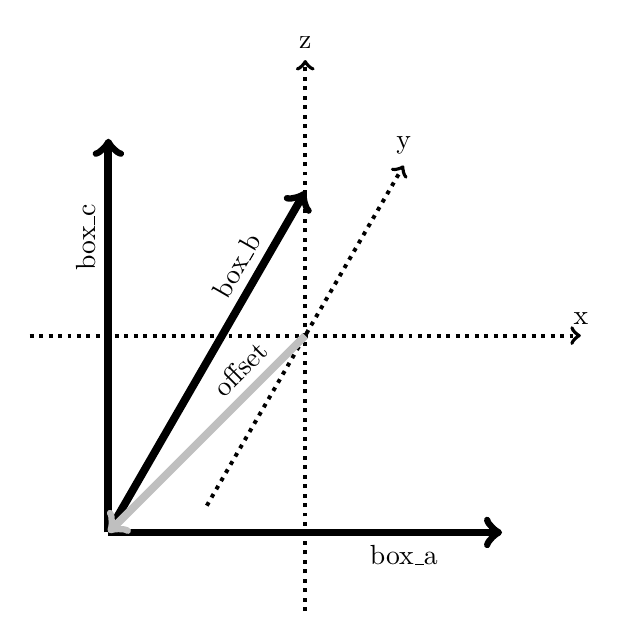
\begin{tikzpicture}
      \draw[->,black,line width=1mm] (-2.5,-2.5) -- (-2.5,2.5) node [near end,above,rotate=90] {box\_c};
      \draw[->,black,line width=1mm] (-2.5,-2.5) -- (0,1.83) node [near end,above,rotate=60] {box\_b};
      \draw[->,black,line width=1mm] (-2.5,-2.5) -- (2.5,-2.5) node [near end,below] {box\_a};

      \draw[->,black,dotted,line width=0.5mm] (-3.5,0) -- (3.5,0) node [left,above] {x};
      \draw[->,black,dotted,line width=0.5mm] (0,-3.5) -- (0,3.5) node [left,above] {z};
      \draw[->,black,dotted,line width=0.5mm] (-1.25,-2.16) -- (1.25,2.16) node [left,above] {y};

      \draw[->,lightgray,line width=1mm] (0,0) -- (-2.5,-2.5) node [near start,above,black,rotate=45] {offset};
\end{tikzpicture}
\end{center}
\caption{Scheme of system parameters describing the form and position of the simulation box}
\label{fig:interface_box_scheme}
\end{figure}

The common setup requires basic data about the simulation system. An overview can be seen in table \ref{tab:fcs_set_common_parameters}. The box vectors
describe the form of the box, in which the particles reside. For each solver there can be certain restrictions as for which kind of systems they can simulate. 
To get an idea which solvers work best (or work at all) with which systems please refer to the corresponding solver description within this documentation.
In general no solver is able to handle non-orthogonal boxes as of yet, although the interface should be able to handle these kind of boxes. The offset
enables the library to handle systems, which are shifted from the coordinate origin. For a graphical scheme, please refer to figure \ref{fig:interface_box_scheme}.
The use of periodicity is likewise restricted as the box forms. Not every solver is able to cope with every combination of periodicity. The only
common parameter not related to the system is the near field flag, which determines whether a method should perform its near field computations by itself or not.
By default, all solvers compute the interactions entirely by themselves. However, some solvers provide the possibility to delegate their near field 
computations to the main program. If the near field flag is set to false (i.e. 0), then interactions inside a solver-specific cutoff range are not computed.
The cutoff range can be retrieved (set) with a separate getter (setter) function. The solver methods provide separate potential functions for performing their
near field computations in the main program. The functionality of the near field flag is currently supported by methods \pthreem and \ptwonfft.

\begin{table}
\begin{center}
\begin{tabular}{|p{0.2\textwidth}|p{0.45\textwidth}|p{0.25\textwidth}|}
          \hline
          parameter name        &       description                                         &   valid values                        \\
          \hline
          handle                &       pointer to parameter containing structure           &   FCS (C) or type (c\_ptr) (Fortran)   \\
          \hline
          near\_field\_flag    &       leave the near field calculations to the library    &   true ($\neq 0$) / false ($0$)       \\
          \hline
          box\_a                &       first vector describing the system box              &   $\in \mathbb{R}^3$                  \\
          \hline
          box\_b                &       second vector describing the system box             &   $\in \mathbb{R}^3$                  \\
          \hline
          box\_c                &       third vector describing the system box              &   $\in \mathbb{R}^3$                  \\
          \hline
          offset                &       offset of the lower front left corner from $\Vect{0}$&   $\in \mathbb{R}^3$                  \\
          \hline
          periodicity           &       periodicity of the system in each dimension (x,y,z) &   true / false                        \\
          \hline
          total\_particles      &       total amount of particles in the system             &   $\in \mathbb{N}^+$                  \\
          \hline 
\end{tabular}
\end{center}
\caption{Parameters for fcs\_common\_set}
\label{tab:fcs_set_common_parameters}
\end{table}

To change the solver-specific parameters, there are solver-specific setter functions. These are called \textit{fcs\_$<$solver$>$\_set\_$<$parameter$>$} where 
\textit{$<$solver$>$} is the abbreviation of the solver (table \ref{tab:solver_overview}) and parameter the name of the relevant parameter. If one wishes to change all parameters of
a solver, the use of \textit{fcs\_$<$solver$>$\_setup} is advised. A list of solver-specific parameters, that can be changed and possible values are available
in the chapters describing the solvers.

\subsection{Tuning Step}
\label{sec:tune_step}
\functiontoindex{fcs\_tune}



Most of the methods need a tuning step in which internal data structures are created according to the actual system that is simulated. Other methods
need information about the distribution of the particles within the system and between the processes. Therefore the tuning step is mandatory. In order
to tune the methods, the user has to call the function \textit{fcs\_tune} with the function call described in figure (\ref{fig:fcs_tune}). The function
calls awaits several input parameters and is similar to the function call of \textit{fcs\_run} described in the following section. First parameter of the
tuning is the handle, which was created in \textit{fcs\_init} (\ref{sec:init_step}) and then filled with \textit{fcs\_common\_set} (\ref{sec:par_setup}).
The parameter \textit{n\_locp} gives the number of particles on the local process, which is identical to the length of the array given as parameter 
\textit{charges}. For the array containing the charges, an array with thrice the length has to be supplied as parameter \textit{charges}. As final parameter,
the parameter \textit{n\_maxlocp} gives an estimation of the maximum number of particles being stored on the local process before the next call of the tuning
routine.\\
This routine is mandatory to be called, in order to grant a unified interface for the library. Some methods, e.g. PEPC, do not need this tuning step. But to be
able to switch the methods within a code without the need to greatly modify the code again, the tuning routine has to be called. If the user wants to use e.g. PEPC
as well as e.g. \ptwonfft, he can use the same program (except for the method-specific setter routines), when including the tuning routine. 

\subsection{Calculation Step}
\label{sec:run_step}
\functiontoindex{fcs\_run}



The calculation step is the centerpiece of the library. Within it, the actual calculation of Coulomb interactions takes place. As mentioned in the description of tuning step,
the call to \textit{fcs\_run} (fig. \ref{fig:fcs_run}) is nearly the same, as for \textit{fcs\_tune} (see \ref{sec:tune_step}). There are two additional parameters, which are \textit{field} and
\textit{potential}. The first is the array to which the field data is added and has a size of thrice the number of local particles (\textit{n\_locp}), the latter
is the array in which the corresponding potentials are saved and has a size equal to the number of local particles (\textit{n\_locp}). All the other parameters
are equal to the parameters of \textit{fcs\_tune} (see above).


\subsection{Clean Up Step}
\label{sec:clean_up_step}
\functiontoindex{fcs\_destroy}



After the calculations are done, the memory allocated by the methods needs to be freed again. This task is done by the function \textit{fcs\_destroy} (fig. \ref{fig:fcs_destroy}).
As parameters only the FCS object is needed, in order to free memory allocated in connection with it, since the internal data structures of the methods are
administrated by those. The call to fcs\_destroy is not mandatory but the user is advised to call it, especially if he or she wants to repeat the calculation
with another method without restarting the program, since it cannot be guaranteed that more then one method can be used simultaneously without memory problems. 

\section{Error Handling}
\label{sec:error_handling}
\index{error handling}

Within the ScaFaCoS library a FCSResult type is defined. With this type return values and error messages of the methods and the interface routines are handled.
The type includes up to three pieces of information about error that have occurred during a call to a ScaFaCoS function. These pieces are a return code, an error
message and the source of the error within the library. As return values the values given in table \ref{tab:c_macros_error} can occur. In order to simplify the
error handling for the ScaFaCoS routines, the routines return \textit{NULL} as return value, instead of an allocated error object containing \textit{FCS\_SUCCESS}
as return value. The other information contained in the error type gives more information about the kind of error that occurred, e.g. if a method cannot handle
a certain system due to restrictions on periodicity, and where the error occurred within the library since the error can happen in functions called inside the
routine called by the user.\\
To get the information out of the error type, there are three functions for this task. Their calls are shown in figures \ref{fig:fcsResult_getReturnCode} to \ref{fig:fcsResult_getErrorSource}.
Due to restrictions in Fortran the message length in Fortran is capped to 256 characters.

\section{Fortran Specifics}

\begin{figure}[htb]
\begin{lstlisting}[language=Fortran,frame=trBL,breaklines,basicstyle=\small,prebreak={\raisebox{0ex}[0ex][0ex]{\ensuremath{\hookleftarrow}}}]
! Fortran
use iso_c_binding
character(kind = c_char, len = 32) :: string = "test_string"
string = trim(adjustl(string)) // c_null_char
\end{lstlisting}
\caption{Example for string truncation for strings used with ScaFaCoS}
\label{fig:example_string_fortran2c}
\end{figure}


In this section some advises are given for Fortran programmers. Since the Fortran interface is a wrapper interface above the C version of the interface trying to
stay as true to the C interface as possible, some things have to be observed. First it is advised to use the interoperable Fortran kinds delivered by the
library, which are \textit{fcs\_integer\_kind\_isoc} for integer and \textit{fcs\_real\_kind\_isoc}. With the usage of these kinds problems concerning the 
interoperability of the values is avoided. Secondly strings have to be terminated with C null characters and have to be trimmed to the correct length. An
example how this can be achieved is given in figure \ref{fig:example_string_fortran2c}. A third difference from Fortran to C is that in the Fortran interface
wherever possible the logical type is used instead of an integer value in C. This is true for every manual setter and getter connected to flags. In the parser
this exchange was not possible (see \ref{sec:interface_parser}).


\section{Further Functionality}

This sections describes some of the functionality the ScaFaCoS library has, which exceeds the pure calculation of Coulomb interactions. It also describes the
output functions within the library and the parser for parameters.

\label{sec:interface_functions}
\subsection{Near Field Solver}
\index{near field solver}
\label{sec:near_field_solver}

\todo[inline]{Should the near field solver be available to the user?}
Within the library a near field solver for given near field potentials is included. Some of the methods (\ptwonfft and \pthreem) need to calculate separate near field
interactions, which is done by this solver. The solver uses a linked cell scheme for fast interaction calculation and uses the sorting library to create and
duplicate the particles (ghost-particles). It is able to handle periodicity and linked cell sizes that are smaller than the cut-off radius. With the near field
flag described in section \ref{sec:par_setup} the calculation of the near field portions of the Coulomb interactions can be delegated to external routines.
In order to do this the methods which support this (currently \pthreem and \ptwonfft) provide a functions which can then be called from the user's program to calculate the
corresponding near field portions of the Coulomb interactions (see figure \ref{fig:fcs_compute_near_field} to \ref{fig:fcs_compute_near}). The aforementioned
functions are generic function that will calculate the according values for the chosen method. It is possible to check if the chosen method is able to relegate
the near field calculation by use of \textit{fcs\_method\_has\_near} (\ref{fig:fcs_method_has_near}).

\subsection{Optional Results}

It is possible to get additional results from the solver concerning the calculation. As of now the only additional result to have is the system virial. It is
possible that some solvers add additional optional results in the future. Since now only the virial is available here will be explained how to get the virial
from the solvers. For that two functions are needed, \textit{fcs\_require\_virial} (\ref{fig:fcs_require_virial}) and \textit{fcs\_get\_virial} (\ref{fig:fcs_get_virial}).
With \textit{fcs\_require\_virial} the user activates or deactivates the calculation of the virial. If set to true, the virial is activated, else it is not
calculated. If it is calculated, the user can get the calculated by the use of \textit{fcs\_get\_virial}. For that he has to pass an allocated array of nine
\textit{fcs\_float} values to the function.\\
Possibly in the next future other optional results will be implemented, if required by the community.

\subsection{Output of Interface Parameters}
\index{parameter output}
\functiontoindex{fcs\_printHandle}

For debugging purposes it is possible to print out the content of the FCS object. This is done by the use of the function \textit{fcs\_printContent} (figure \ref{fig:fcs_printHandle}).
The output shows the current values of the parameters set within the FCS object. If no changes were made to the solver-specific parameters, it shows the default
values for them. The behavior of the routine if used on a freshly created FCS object without set common parameters is undefined.

\subsection{Parser}
\index{parser}
\functiontoindex{fcs\_parser}
\label{sec:interface_parser}

To simplify the parameter input for programs basing on script file input, the ScaFaCoS library offers a parser that allows to read in parameters from a string.
The format of the passed string must adhere to the example shown in figure \ref{fig:parser_example}, while the function call can be seen in figure \ref{fig:fcs_parser}

\begin{figure}[htb]
\begin{lstlisting}[language=Fortran,frame=trBL,breaklines,basicstyle=\small,prebreak={\raisebox{0ex}[0ex][0ex]{\ensuremath{\hookleftarrow}}}]
string = "box_a,1.0,0.0,0.0,near_field_flag,1,pepc_theta,0.3"
\end{lstlisting}
\caption{Example of a parser string setting the first box vector, the near field flag and a method-specific parameter.}
\label{fig:parser_example}
\end{figure}

The format is an alteration of parameter name and value(s). In the example the first parameter to be set is a generic one, so no prefix is needed and the parameter
name is \textbf{box\_a}. Since the first box vector needs three floating point values, these are given after the parameter name, always separated by commas.
After the final parameter value, the next parameter name is expected, in the case of the example the parameter is another generic one, the \textbf{near\_field\_flag}.
Because this parameter needs only one integer value, it given and immediately followed by the next parameter name. The last parameter to be set is a solver-specific
one, the parameter \textbf{theta} from the PEPC solver. Since it is a PEPC-specific parameter, the solver name is added as a prefix, followed by the parameter name.
After it the parameter value follows, like with the generic parameters.\\
For Fortran users the advise, that every flag which is set with the parser, has to used the C syntax which requires an integer value (0 for false, 1 for true) instead
of \textit{.true.} or \textit{.false.}.

\FloatBarrier
\renewcommand\arraystretch{1.0}

\input{fmm} 
\input{memd}
\input{mmm1d}
\input{mmm2d}
\chapter{Ewald}
\label{cha:ewald}

\solvertoindex{Ewald}

%%% Local Variables: 
%%% mode: latex
%%% TeX-master: ug.tex
%%% End: 

The well-known Ewald formula for the computation of \eqref{eq:ewald_potential} splits the
electrostatic potential $\phi$ into the following parts
\begin{equation}\label{eq:ewald}
 \phi = \phi^{\text{real}} + \phi^{\text{reci}}  + \phi^{\text{self}}  + \phi^{\text{dipo}},
\end{equation}
where the contribution from real space $ \phi^{\text{real}}$, reciprocal space $\phi^{\text{reci}}$,
the self-energy $\phi^{\text{self}}$ and the dipole correction $\phi^{\text{dipo}}$ are given by
\begin{eqnarray}
  \phi^{\text{real}}(\mathbf x_j)
  &=& \nonumber
    \sum_{\mathbf r\in \mathbb Z^3}
    \underset{ l\neq j \,{\text{for}}\, \mathbf r= \mathbf 0}{\sum_{l=1}^M}
    q_l\frac{{\text{erfc}}(\alpha \|\mathbf x_j -\mathbf x_l +\mathbf r B\|_2)}{\|\mathbf x_j -\mathbf x_l +\mathbf r B\|_2},\\
  \phi^{\text{reci}}(\mathbf x_j)
  &=& \label{eq:ewald_reci}
    \frac{1}{\pi B} \sum_{\mathbf k\in \mathbb Z^3\setminus\{\mathbf 0\}}
    \frac{{\text{e}}^{-\pi^2 \|\mathbf k\|_2^2/(\alpha B)^2}}{\|\mathbf k\|_2^2}
    \sum_{l=1}^M q_l {\text{e}}^{-2\pi \text{i} \mathbf k (\mathbf x_j -\mathbf x_l)/B}\, ,\\
  \phi^{\text{self}} (\mathbf x_j)
  &=&
    -2 q_j \frac{\alpha}{\sqrt{\pi}}\; ,\nonumber  \\
  \widetilde\phi^{\text{dipo}}
  &=&
    \frac{2\pi}{3V}\bigg(\sum_{l=1}^Mq_{l}\mathbf x_{l}\bigg)^{2}\; .\nonumber %\label{eq:E_dipol_part}
\end{eqnarray}
Thereby, the complementary error function is defined by $\textrm{erfc}(z) =
\frac{2}{\sqrt{\pi}}\int_z^\infty \text{e}^{-t^2} \text{d}t$.
Choosing optimal parameters, Ewald summation scales as ${\cal O}(M^{3/2})$ \cite{kolafa92a}.

\chapter{\ptwonfftcap -- Particle-Particle NFFT}
\label{cha:p2nfft}

\solvertoindex{\ptwonfft}
\solvertoindex{Particle-Particle NFFT}

\def\alp{13}


%%% Local Variables: 
%%% mode: latex
%%% TeX-master: ug.tex
%%% End: 


\ptwonfft is a common framework for almost all FFT based fast Coulomb solvers.
The computation of Coulomb interactions is split into a short range interaction (near field) and
a long range interaction (far field).
For sake of simplicity, we describe the idea of \ptwonfft only for the one-dimensional case.
In addition, we do not stress all the details, that arise from the difference between periodic and
non-periodic boundary conditions. More detailed descriptions of the algorithms can be found in \cite{PiPo10}.

\section{Description of the Method}

As usual, we assume $M$ charges $q_l$ at position $r_l$. The potentials $\phi_j$ at position $r_j$
are given by
\begin{equation*}
  \phi_j
  =
  \sideset{}{^\prime}\sum_{l=1}^M
    q_l\frac{1}{r_{jl}}
  \,,
\end{equation*}
and the Electrostatic fields $E_j$ at position $r_j$ are given by
\begin{equation*}
  E_j
  =
  \sideset{}{^\prime}\sum_{l=1}^M
    q_l\nabla\frac{1}{r_{jl}}
  =
  \sideset{}{^\prime}\sum_{l=1}^M
    q_l \frac{r_l}{r_{jl}}
  \,.
\end{equation*}
Hereby, the distance between two particles at positions $r_j$ and $r_l$ is given by $r_{jl}:=|r_j-r_l|$.

\subsection{Periodic boundary conditions}
In this section we present a straightforward method, that accelerates the traditional Ewald
summation technique by NFFT. This combination was first presented in \cite{HeLa06} and
is very similar to the FFT-accelerated Ewald sums, namely, the so-called
particle-particle particle-mesh (P$^3$M), particle-mesh Ewald (PME) and smooth particle-mesh
Ewald (SPME), see also \cite{DeHo98a}.
Additionally we will see, that the accelerated Ewald summation can be reinterpreted
into a method very similar to our fastsum Algorithm~\ref{algo:fastsum}.


In order to overcome this increase in time we apply the NFFT for the calculation of the
reciprocal-space potential  $\phi^{\rm reci}$ and we obtain a method similar as our fast summation method.
To this end, we compute the Fourier transformed charge density
\begin{equation*}
 S(\mathbf k) = \sum_{l=1}^M q_l {\rm e}^{+2\pi {\rm i} \mathbf k \mathbf x_l/B}
\end{equation*}
by NFFT$^\adj$ and after truncation of the sum \eqref{eq:ewald_reci} we obtain by NFFT
\begin{equation*}
 \phi^{\rm reci}(\mathbf x_j) \approx
 \frac{1}{\pi B} \sum_{\mathbf k\in I_{\mathbf N}\setminus\{\mathbf 0\}}
 \frac{{\rm e}^{-\pi^2 \|\mathbf k\|_2^2/(\alpha B)^2}}{\|\mathbf k\|_2^2}
 S(\mathbf k){\rm e}^{-2\pi {\rm i} \mathbf k \mathbf x_j/B}\, .
\end{equation*}





\subsection{Calculation of the Potentials}

\begin{figure}[htb]
  \centering
  \beginmypgfhack{p2nfft_ewald_split}
%   \beginpgfgraphicnamed{p2nfft_ewald_split}
  \begin{tikzpicture}
    \node (plot_one_over_r) [right]{
      \begin{tikzpicture}
        \begin{axis}[tiny, xmin=0, xmax=0.5, ymin=0, ymax=17]
          \addplot gnuplot [id=erf,mark=none,domain=0:0.5, samples = 101, very thick, black]{(x==0) ? 100 : 1/x};
        \end{axis}
      \end{tikzpicture}
    };
    \node (plot_equals) at (plot_one_over_r.east) [right]{=};
    \node (plot_erfc) at (plot_equals.east) [right]{
      \begin{tikzpicture}
        \begin{axis}[tiny, xmin=0, xmax=0.5, ymin=0, ymax=17]
          \addplot gnuplot [id=erf,mark=none,domain=0:0.5, samples = 101, very thick, black]{(x==0) ? 100 : 1/x};
          \addplot gnuplot [id=erf,mark=none,domain=0:0.5, samples = 101, very thick, blue]{(x==0) ? 100 : erfc(x*\alp)/x};
        \end{axis}
%         \node [xshift=8ex, yshift=9ex] {\tiny$\alpha=\alp$};
      \end{tikzpicture}
    };
    \node (plot_plus) at (plot_erfc.east) [right]{+};
    \node (plot_erf) at (plot_plus.east) [right]{
      \begin{tikzpicture}
        \begin{axis}[tiny, xmin=0, xmax=0.5, ymin=0, ymax=17]
          \addplot gnuplot [id=erf,mark=none,domain=0:0.5, samples = 101, very thick, black]{(x==0) ? 100 : 1/x};
          \addplot gnuplot [id=erf,mark=none,domain=0:0.5, samples = 101, very thick, red]{(x==0) ? 2*\alp/sqrt(pi) : erf(x*\alp)/x};
        \end{axis}
%         \node [xshift=8ex, yshift=9ex] {\tiny$\alpha=\alp$};
      \end{tikzpicture}
    };
    \node (eqn_one_over_r) at (plot_one_over_r.north) [above]{
      $\tfrac{1}{r}$
    };
    \node (eqn_erfc) at (plot_erfc.north) [above]{
      \color{blue}$\tfrac{1}{r} - R(r)$
    };
    \node (eqn_erf) at (plot_erf.north) [above]{
      \color{red}$R(r)$
    };
    \node (eqn_equals) at (plot_equals.north) [above=7ex]{=};
    \node (eqn_plus) at (plot_plus.north) [above=7ex]{+};
  \end{tikzpicture}
  \endmypgfhack
%   \endpgfgraphicnamed
  \caption{Splitting of Coulomb potential into near field (blue) and far field (red).}
\end{figure}

\begin{equation*}
  \phi(r_j)
  =
  \sideset{}{^\prime}\sum_{l=1}^M
    \frac{q_l}{r_{jl}}
  =
  R(0) + \sideset{}{^\prime}\sum_{l=1}^M
    q_l \left( \frac{1}{r_{jl}} - R(r_{jl}) \right)
  - \sum_{l=1}^M
    q_l R(r_{jl})
  \,,\quad j=1,\hdots,M
\end{equation*}



\begin{equation*}
  R(r)
  \approx
    \sum_{k=-N/2}^{N/2-1} \hat R_k \eim{kr}
\end{equation*}

\begin{equation*}
  \sum_{l=1}^M
    q_l R(r_{jl})
  \approx
  \sum_{l=1}^M q_l
    \sum_{k=-N/2}^{N/2-1} \hat R_k \eim{kr_{jl}}
  =
  \sum_{k=-N/2}^{N/2-1} \hat R_k
    \left(
      \sum_{l=1}^M q_l \eip{kr_l}
    \right)
    \eim{kr_j}
\end{equation*}

Near field interactions are computed with the ScaFaCoS near field solver, but can also be redirected to any other the near field solver.

Far field interactions are computed via convolution in Fourier space.
With the appropriate choice of window functions and convolutions in Fourier space,
\ptwonfft becomes the P3M (default for fully periodic boundaries), the NFFT based fast summation (default for fully non-periodic boundaries)
or almost any other FFT based fast Coulomb solver like PME, SPME, Gaussian split Ewald or plain Ewald summation.
Note, that an uniform particle distribution is required in order to achieve the typical $\mathcal{O}(N\log N)$ scaling.

\subsection{Calculation of the Electrostatic Fields}

\subsection{Calculation of the Virial}






\newpage
\section{Features}

\begin{description}
\item[Periodicity:] Only fully periodic and fully non-periodic boundaries are supported.
\item[Box shape:] Only cubic box shape is supported.
\item[Autotuning:] For fully periodic boundaries, the parameters can be automatically tuned when a
  required tolerance in the absolute rms field error is provided. For fully non-periodic boundaries,
  the parameters are more or less intelligently guessed when a required tolerance in the absolute
  potential error is provided.  
\item[Delegate near-field:] Yes.
\item[Virial:] Yes for fully non-periodic boundaries. For fully periodic boundaries we only compute an approximation of
  the diagonal of the virial tensor, \ie, all entries of the diagonal are set equal to one third of the total energy.
\end{description}

\section{Solver-specific Parameters}
The tolerance parameters are common to all ScaFaCoS solvers. At the moment \ptwonfft only supports automatic parameter tuning for the following tolerance types.
\begin{itemize}
  \item \verb!tolerance_type! -
    The type of error that we want to check for. Allowed values are \verb!FCS_TOLERANCE_TYPE_FIELD! (absolute rms error in the fields)
    for fully periodic boundaries and \verb!FCS_TOLERANCE_TYPE_POTENTIAL! (absolute rms error in the potentials) for non-periodic boundaries.
  \item \verb!tolerance! -
    The allowed tolerance of the error. Type of the error is given by \verb!tolerance_type!. If the required tolerance can't be achieved
    with the given parameters, \ptwonfft aborts with an error message.
\end{itemize}

In addition, \ptwonfft offers the following parameters, which can be adjusted by the \ptwonfft-specific functions described in the next section.
Alternatively, you can use the ScaFaCoS test program together with the optional command line argument \verb!-c! and a comma separated list
of parameter settings, e.g., use
\begin{verbatim}
./scafacos_test p2nfft systems/3d-periodic/cloud_wall.xml.gz \
-c tolerance_field,1e-4,p2nfft_r_cut,4.5,pnfft_N,16,16,16,pfft_patience,0
\end{verbatim}
in order to run the test program with a near field cut off range of $4.5$ and a sloppy planned FFT of size $16\times 16 \times 16$ up to tolerance $10^{-4}$ in the fields.
\begin{itemize}
  \item \verb!p2nfft_r_cut! -
    Absolute cutoff distance of the near field. Can be automatically tuned.
    Feasible values are any positive floats. Especially, \ptwonfft still works correct if \verb!p2nfft_r_cut! exceeds the simulation box.
    We do not require that \verb!p2nfft_r_cut! has to be less than half the smallest simulation box length.
    When \verb!p2nfft_r_cut! is chosen too small, the errors of the algorithm become large,
    the required accuracy might not be achieved, or the grid has to be chosen very large, which will slow down the algorithm.
    When \verb!p2nfft_r_cut! is chosen too large, the algorithm might become slow as most computation is done in the near field region.
    This parameter corresponds to \verb!r_cut! of the P3M solver.
  \item \verb!p2nfft_epsI! -
    Relative cutoff distance of the near field. \ptwonfft scales the original box size into a cube of side length 1.
    For fully periodic boundary conditions this corresponds to a simple scaling by the box size. However, the scaling is more complicated if non-periodic
    boundary conditions are involved. Application of the same scaling factor on \verb!r_cut! gives \verb!epsI!.
    Feasible values are any positive floats that fulfill $\verb!epsI! < 0.5$.
  \item \verb!p2nfft_epsB! -
    Regularization border for \ptwonfft with non-periodic boundary conditions. This parameter corresponds to the rescaled system into a unit cube of side length 1.
    Feasible values are any positive floats that fulfill $\verb!epsI! + \verb!epsB! < 0.5$.
    This parameter does not have any effect for fully periodic boundary conditions. Default value is $\verb!epsB! := \verb!epsI!$.
  \item \verb!p2nfft_k_cut! -
    Spherical cutoff distance in Fourier space. If this parameter is set to a positive float $k_c>0$, all Fourier coefficients $\hat f_{\mathbf k}$ with
    $\|\mathbf k\|_2 > kc$ will be set to zero, i.e., the approximation in Fourier space uses a spherical cutoff scheme.
    This is usefull, e.g., for comparision of results to classical Ewald summation.
    Feasible values are any positive float (enable spherical cutoff) or any negative float (disable spherical cutoff).
    The spherical cutoff is not applied per default, since FFTs naturally use a box shaped cutoff scheme.
  \item \verb!p2nfft_alpha! -
    Ewald splitting parameter. Can be automatically tuned.
    This parameter corresponds to \verb!alpha! of the P3M solver.
  \item \verb!p2nfft_cao! -
    Charge assignment order. Can be automatically tuned. This parameter mostly corresponds to \verb!cao! of the P3M solver.
    However, note that this is only a wrapper that sets \verb!pnfft_m! to the value \verb!(p2nfft_cao+1)/2! (division rounded down).
    Therefore, \ptwonfft will always use an even charge assignment order.
  \item \verb!p2nfft_intpol_order! -
    \ptwonfft uses interpolation tables to speed up the repeated computation of the near field correction. The order of interpolation is given by \verb!intpol_order!.
    Feasible values are $-2$ (approximation of the error function according to \cite[eq.~(7.1.26)]{AbSt72}, which yields an error of $1.5\times 10^{-7}$),
    $-1$ (direct evaluation of the error function), $0$ (constant interpolation), $1$ (linear interpolation), $2$ (quadratic interpolation) and $3$ (cubic interpolation).
    Default value is $3$.
  \item \verb!p2nfft_reg_near! -
    Choose between the two near field regularization methods for non-periodic boundaries. Feasible values are $0$ (Fourier coefficients have been precomputed via CG iteration, only available for some sets of parameters)
    and $1$ (Regularization with two-point Taylor polynomials). Default value is $0$, if possible.
  \item \verb!p2nfft_reg_near_name! (alternative: \verb!p2nfft_reg_near!) -
    Choose between the two regularization methods for non-periodic boundaries. Feasible values are \verb!cg! (Fourier coefficients have been precomputed via CG iteration, only available for some sets of parameters)
    and \verb!t2p! (Regularization with two-point Taylor polynomials). Default is \verb!cg!, if possible.
  \item \verb!p2nfft_reg_far! -
    Choose between the available regularization methods at the far field boundary for non-periodic boundaries.
    Feasible values are $0$ (Fourier coefficients have been precomputed via CG iteration, only available for some sets of parameters and only available in combination with the flag \verb!rad_cg! for near field regularization),
    $1$ (Regularization with two-point Taylor polynomials and explicitly chosen constant continuation value), and
    $2$ (Regularization with two-point Taylor polynomials and implicitly chosen constant continuation value). Default value is $2$.
  \item \verb!p2nfft_reg_far_name! (alternative: \verb!p2nfft_reg_far!) -
    Choose between the two regularization methods for non-periodic boundaries. Feasible values are \verb!rad_cg! (radial regularization based on the \verb!cg! near field regularization, only available for some sets of parameters),
    \verb!rad_t2p_sym! (radial regularization with symmetric two-point Taylor polynomial),
    \verb!rad_t2p_ec!  (radial regularization with two-point Taylor polynomial and explicitly chosen constant continuation value),
    \verb!rad_t2p_ic!  (radial regularization with two-point Taylor polynomial and implicitly chosen constant continuation value),
    \verb!rec_t2p_sym! (radial regularization with symmetric two-point Taylor polynomial),
    \verb!rec_t2p_ec!  (radial regularization with two-point Taylor polynomial and explicitly chosen constant continuation value), and
    \verb!rec_t2p_ic!  (radial regularization with two-point Taylor polynomial and implicitly chosen constant continuation value).
    Default value is \verb!rad_t2p_ic!.
  \item \verb!p2nfft_c! -
    The constant continuation value of the far field regularization. This parameter only takes affect, if far field regularization \verb!rad_t2p_ec! or \verb!rec_t2p_ec! is enabled.
    Feasible values are any floating point numbers. Default value is $0.0$.
  \item \verb!p2nfft_p! -
    The degree of the two-point Taylor polynomial. This parameter only takes affect, if regularization \verb!t2p! has been enabled.
    Feasible values are any integers between $1$ and $16$. Default value is $7$.
  \item \verb!p2nfft_require_virial! -
    Decide if the computation of the virial should be included in \ptwonfft.
    Feasible values are $0$ (disable virial computation), or any other integer (enable virial computation).
    Default value is $0$ (disable virial computation).
  \item \verb!p2nfft_ignore_tolerance! -
    On default, \ptwonfft aborts with an error message, if the required error tolerance can not be reached.
    This flag disables the check for accuracy and gives the possibility to run \ptwonfft
    with any set of parameters. It is intended for very experienced users that tune all parameters manually.
    Default value is $0$ (abort if tolerance check fails). Any other value disables the tolerance check.
  \item \verb!p2nfft_verbose_tuning! -
    Decide if a full list of \ptwonfft parameter settings is printed on stdout or not.
    Feasible values are $0$ (do not print), or any other integer (print the parameters).
    The default value is $1$ if \project was configured with the \verb+--enable-fcs-info+ flag, and $0$ otherwise.
\end{itemize}

\subsection{PNFFT-specific Parameters}
\begin{itemize}
  \item \verb!pnfft_N! (acronym: \verb!p2nfft_grid!) -
    Size of the FFT grid. Can be automatically tuned.
    Feasible values are three comma separated, even, positve integers, e.g., \verb!pnfft_N,16,32,12!.
    Optimal values are in the order of $M^{1/3}$, \ie, one grid point for each particle.
    The grid size may be any even, positive integer, but powers of
    two are recommended. The larger the grid, the smaller the
    error, but also the higher the memory and computational requirements
    of the algorithm.
    This parameter corresponds to the FFT grid size (\verb!grid!) of the P3M solver.
  \item \verb!pnfft_n! (acronym: \verb!p2nfft_oversampled_grid!) -
    Size of the oversampled FFT grid. Can be automatically tuned.
    Especially for non-periodic boundaries it is necessary to introduce oversampling to reduce the aliasing error.
    Feasible values are three comma separated, even integers with $\verb!n! \ge \verb!N!$ in every dimension, e.g., \verb!pnfft_N,16,32,12,pnfft_n,20,64,12!.
    Default value is \verb!N! for fully periodic boundaries and 2\verb!N! for fully non-periodic
    boundaries.
  \item \verb!pnfft_window! (alternative: \verb!pnfft_window_name!) -
    NFFT window function. Feasible values are $0$ (Kaiser-Bessel window), $1$ (Gaussian window),
    $2$ (B-spline window), $3$ (Sine Cardinal window - Fourier transform of the B-spline window) and $4$
    (window function based on the modified Bessel function of first kind - Fourier transform of the Kaiser-Bessel window).
    Default value is $2$ (B-spline). Recommended values are $0$ (Kaiser-Bessel) for fully non-periodic boundaries and $2$ (B-spline) for fully periodic boundaries.
  \item \verb!pnfft_window_name! (alternative: \verb!pnfft_window!) -
    Name of the NFFT window function. Feasible values are \verb!kaiser! (Kaiser-Bessel window), \verb!gaussian! (Gaussian window),
    \verb!bspline! (B-spline window), \verb!sinc! (Sine Cardinal window - Fourier transform of the B-spline window) and \verb!bessel_i0!
    (window function based on the modified Bessel function of first kind - Fourier transform of the Kaiser-Bessel window).
    Default value is \verb!bspline!. Recommended values are \verb!kaiser! for fully non-periodic boundaries and \verb!bspline! for fully periodic boundaries.
  \item \verb!pnfft_m! (see also: \verb!p2nfft_cao!) -
    Real space cutoff of the window function. The number of grid points that are influenced
    by a charged particle. Can be automatically tuned. Allowed values are any positive integers.
    In most cases \verb!m! is chosen between $1$ (low precision) and $16$ (very high precision).\\
    {\bfseries Note: Due to historical reasons, this parameter corresponds to one half of the charge assignment order
    (\verb!cao!) of the P3M solver!}
  \item \verb!pnfft_b! -
    Shape parameter of the NFFT window function corresponding to the three dimensions. Can be automatically tuned.
    Feasible values are three comma separated positiv floating point numbers, e.g., \verb!pnfft_b,0.5,1.0,3.2!.
    Choosing an optimal value for b is not that easy but influences the error a lot.
    Therefore, you should only change the default value if you know what you do.
  \item \verb!pnfft_intpol_order! -
    PNFFT uses interpolation tables to speed up the repeated evaluation of the window functions. The integer \verb!pnfft_intpol_order! gives the interpolation order.
    Feasible values are $-1$ (direct evaluation of window function without interpolation), $0$, (constant interpolation), $1$ (linear interpolation), $2$ (quadratic interpolation) and $3$ (cubic interpolation).
    Default value is $3$ (cubic interpolation).
  \item \verb!pnfft_direct! -
    Flag to enable plain NDFT instead of the fast approximative NFFT algorithms. 
    Feasible values are $0$ (use NFFT), or any other integer \verb!pnfft_direct!$\ne0$ (use NDFT). Default value is \verb!pnfft_direct!$=0$ (use NFFT).
  \item \verb!pnfft_pre_phi_hat! -
    Flag to enable precomputed Fourier coefficients for faster computation of the diagonal matrix in the NFFT algorithm.
    Feasible values are $0$ (turn off pre-computation), or any other integer \verb!pnfft_pre_phi_hat!$\ne0$ (enable pre-computation).
    Default value is $1$ (enable pre-computation).
  \item \verb!pnfft_fg_psi! -
    Set PNFFT flag \verb!PNFFT_FG_PSI!. Only Gaussian window function we can use Fast Gaussian Gridding in order to speed up the evaluation of the window function.
    Feasible values are $0$ (switch Fast Gaussian gridding off), or any other integer \verb!pnfft_fg_psi!$\ne0$ (use Gaussian gridding).
    Default value is $0$ (since B-Spline is the default window function).
  \item \verb!pnfft_fft_in_place! -
    Set PNFFT flag \verb!PNFFT_FFT_IN_PLACE!. This causes the PNFFT planner to use in-place-FFTs, which saves about half of the memory for FFT but may sacrifices some performance.
    Feasible values are $0$ (call out-of-place FFTs), or any other integer \verb!pnfft_fft_in_place!$\ne0$ (call in-place-FFTs).
    Default value is \verb!pnfft_fft_in_place!$=0$ (call out-of-place FFTs).
  \item \verb!pnfft_sort_nodes! -
    Set PNFFT flag \verb!PNFFT_SORT_NODES!. Chooses whether to call a local sort before the interpolation step. This may result in better cache locality.
    Feasible values are $0$ (omit local sort), or any other integer \verb!pnfft_sort_nodes!$\ne0$ (sort before interpolation).
    Default value is \verb!pnfft_sort_nodes!$=0$ (omit local sort).
  \item \verb!pnfft_interlaced! -
    Set PNFFT flag \verb!PNFFT_INTERLACED!. Chooses whether PNFFT uses interlacing. This gives better accuracy at the price of more operations.
    Feasible values are $0$ (omit interlacing), or any other integer \verb!pnfft_interlaced!$\ne0$ (enable interlacing).
    Default value is \verb!pnfft_interlaced!$=0$ (omit interlacing).
  \item \verb!pnfft_grad_ik! -
    Set PNFFT flag \verb!PNFFT_GRAD_IK!. Chooses whether PNFFT computes the gradient through multiplication with $-2\pi\textrm{i}\mathbf{k}$ in Fourier space.
    This gives better accuracy in comparison to analytic differentiation at the price of more operations. Especially, we have to call four backward FFTs (instead of one for analytic differentiation).
    Feasible values are $0$ (use analytic differentiation), or any other integer \verb!pnfft_grad_ik!$\ne0$ (use Fourier space differentiation).
    Default value is \verb!pnfft_grad_ik!$=0$ (use analytic differentiation).
  \item \verb!pnfft_pre_psi! -
    Set PNFFT flag \verb!PNFFT_PRE_PSI!. Tensor product based precomputation of the window function. This option reduces the amount of repeated evaluations of the window function at the cost of
    $6(2m+1)M$ floats (or $3(2m+1)M$ floats if the gradient is not needed).
    Since the this kind of precomputation depends on the nodes $\mathbf x_j$, it must be performed during \verb!fcs_run! instead of \verb!fcs_tune!.
    Feasible values are $0$ (switch off precomputation), or any other integer \verb!pnfft_pre_psi!$\ne0$ (switch on precomputation).
    Default value is $0$ (no precomputation). This flag can not be used together with \verb!pnfft_pre_full_psi!.
  \item \verb!pnfft_pre_fg_psi! -
    Set PNFFT flags \verb!PNFFT_FG_PSI! and \verb!PNFFT_PRE_PSI!, i.e., use Fast Gaussian Gridding for tensor product based precomputation.
    Since the this kind of precomputation depends on the nodes $\mathbf x_j$, it must be performed during \verb!fcs_run! instead of \verb!fcs_tune!.
    Feasible values are $0$ (switch off precomputation), or any other integer \verb!pnfft_pre_fg_psi!$\ne0$ (switch on precomputation).
    Default value is $0$ (no precomputation). This flag can not be used together with \verb!pnfft_pre_full_psi!.
  \item \verb!pnfft_pre_full_psi! -
    Set PNFFT flag \verb!PNFFT_PRE_FULL_PSI!. Full precomputation of the window function. This option reduces the amount of repeated evaluations of the window function at the cost of
    $4(2m+1)^3M$ floats (or $(2m+1)^3M$ floats if the gradient is not needed).
    Since the this kind of precomputation depends on the nodes $\mathbf x_j$, it must be performed during \verb!fcs_run! instead of \verb!fcs_tune!.
    Feasible values are $0$ (switch off precomputation), or any other integer \verb!pnfft_pre_psi!$\ne0$ (switch on precomputation).
    Default value is $0$ (no precomputation). This flag can not be used together with \verb!pnfft_pre_full_psi!.
  \item \verb!pnfft_pre_full_fg_psi! -
    Set PNFFT flags \verb!PNFFT_FULL_FG_PSI! and \verb!PNFFT_PRE_FULL_PSI!, i.e., use Fast Gaussian Gridding for full window function precomputation.
    Since the this kind of precomputation depends on the nodes $\mathbf x_j$, it must be performed during \verb!fcs_run! instead of \verb!fcs_tune!.
    Feasible values are $0$ (switch off precomputation), or any other integer \verb!pnfft_pre_full_fg_psi!$\ne0$ (switch on precomputation).
    Default value is $0$ (no precomputation). This flag can not be used together with \verb!pnfft_pre_psi!.
  \item \verb!pnfft_real_f! -
    Set PNFFT flag \verb!PNFFT_REAL_F!. Normally, PNFFT works on complex valued inputs. This flag enables some optimizations for real valued inputs, e.g., substituting complex additions and multiplications with real ones.
    However, this comes at the price of strided memory access and does not always improve performance.
    Feasible values are $0$ (use complex operations), or any other integer \verb!pnfft_real_f!$\ne0$ (use real operations where possible).
    Default value is \verb!pnfft_real_f!$=0$ (use complex operations).
\end{itemize}

\subsection{PFFT-specific Parameters}
\begin{itemize}
  \item \verb!pfft_patience! -
    Similar to FFTW, the PFFT library splits the computation of parallel FFT into a more or less time consuming planning step and a fast execution step.
    The time spent for planning can be adjusted by the \verb!pfft_patience! flag. Feasible values are $0$ (plan PFFT with \verb!PFFT_ESTIMATE!), $1$ (plan PFFT with \verb!PFFT_MEASURE!),
    $2$ (plan PFFT with \verb!PFFT_PATIENT!) and $3$ (plan PFFT with \verb!PFFT_EXHAUSTIVE!). All other values raise an error. Default value is $1$ (\verb!PFFT_MEASURE!).
  \item \verb!pfft_tune! -
    The PFFT library uses FFTW for computing serial FFTs combined with serial transpositions. Sometimes its better to perform the FFT and transposition in two separate steps,
    but the FFTW planner does not recognize. For value \verb!pfft_tune!$=0$ PFFT uses the FFTW plan as it is. For any other value, PFFT calls an additional planner in order to decide
    if performance gets better when the local FFT and transposition is performed in two separate steps. For large local array sizes this tuning gets very time consuming.
    Default value is $0$ (tuning turned off).
  \item \verb!pfft_preserve_input! -
    PFFT can chose between a larger set of algorithms, if it is allowed to overwrite the input array.
    Feasible values are $0$ (PFFT is allowed to destroy input), or any other integer \verb!pfft_preserve_input!$\ne0$ (PFFT is not allowed to destroy input).
    Default value is $0$ (PFFT is allowed to destroy input).
\end{itemize}


\section{Solver-specific Functions}
\begin{itemize}
  \item
\begin{alltt}
FCSResult fcs_p2nfft_set_r_cut(FCS handle, fcs_float r_cut);
FCSResult fcs_p2nfft_get_r_cut(FCS handle, fcs_float* r_cut);
FCSResult fcs_p2nfft_set_r_cut_tune(FCS handle);
\end{alltt}
    Set/restore/retrieve absolute near field cutoff radius.
  \item
\begin{alltt}
FCSResult fcs_p2nfft_set_epsI(FCS handle, fcs_float eps_I);
FCSResult fcs_p2nfft_get_epsI(FCS handle, fcs_float* eps_I);
FCSResult fcs_p2nfft_set_epsI_tune(FCS handle);
\end{alltt}
    Set/restore/retrieve relative near field cutoff radius.
  \item
\begin{alltt}
FCSResult fcs_p2nfft_set_epsB(FCS handle, fcs_float eps_B);
FCSResult fcs_p2nfft_get_epsB(FCS handle, fcs_float* eps_B);
FCSResult fcs_p2nfft_set_epsB_tune(FCS handle);
\end{alltt}
    Set/restore/retrieve relative far field regularization border.
  \item
\begin{alltt}
FCSResult fcs_p2nfft_set_alpha(FCS handle, fcs_float alpha);
FCSResult fcs_p2nfft_get_alpha(FCS handle, fcs_float* alpha);
FCSResult fcs_p2nfft_set_alpha_tune(FCS handle);
\end{alltt}
    Set/restore/retrieve Ewald splitting parameter.
  \item
\begin{alltt}
FCSResult fcs_p2nfft_set_interpolation_order(
    FCS handle, fcs_int intpol_order);
FCSResult fcs_p2nfft_get_interpolation_order(
    FCS handle, fcs_int* intpol_order);
\end{alltt}
    Set/retrieve interpolation order of near field correction (optional, default = 3).
  \item
\begin{alltt}
FCSResult fcs_p2nfft_set_regularization(FCS handle, fcs_int reg);
FCSResult fcs_p2nfft_get_regularization(FCS handle, fcs_int* reg);
FCSResult fcs_p2nfft_set_regularization_by_name(
    FCS handle, char* reg_name);
\end{alltt}
    Set/retrieve the near field regularization by number or name (default = 0).
    Feasible values are 0 (\verb!"cg"!) and 1 (\verb!"t2p"!).
  \item
\begin{alltt}
FCSResult fcs_p2nfft_set_p(FCS handle, fcs_int p);
FCSResult fcs_p2nfft_get_p(FCS handle, fcs_int* p);
FCSResult fcs_p2nfft_set_p_tune(FCS handle);
\end{alltt}
    Set/restore/retrieve polynomial degree of two-point Taylor regularization.
  \item
\begin{alltt}
FCSResult fcs_p2nfft_require_virial(
    FCS handle, fcs_int require_virial);
\end{alltt}
    Enable virial computation (optional, default = 0).
\begin{alltt}
FCSResult fcs_p2nfft_get_virial(FCS handle, fcs_float* virial);
\end{alltt}
    Retrieve virial (optional, default)
\begin{alltt}
FCSResult fcs_p2nfft_virial_is_active(
    FCS handle, fcs_int* yes_or_no);
\end{alltt}
    Check if virial computation is enabled.
  \item
\begin{alltt}
FCSResult fcs_p2nfft_set_ignore_tolerance(
    FCS handle, fcs_int set_ignore_tolerance);
FCSResult fcs_p2nfft_get_ignore_tolerance(
    FCS handle, fcs_int* set_ignore_tolerance);
\end{alltt}
    Set/retrieve flag for disabling the accuracy check (default = 0).
  \item
\begin{alltt}
FCSResult fcs_p2nfft_set_grid(
    FCS handle, fcs_int N0, fcs_int N1, fcs_int N2);
FCSResult fcs_p2nfft_get_grid(
    FCS handle, fcs_int* N0, fcs_int* N1, fcs_int* N2);
FCSResult fcs_p2nfft_set_grid_tune(FCS handle);
\end{alltt}
    Set/restore/retrieve FFT grid size.
  \item
\begin{alltt}
FCSResult fcs_p2nfft_set_oversampled_grid(
    FCS handle, fcs_int n0, fcs_int n1, fcs_int n2);
FCSResult fcs_p2nfft_get_oversampled_grid(
    FCS handle, fcs_int* n0, fcs_int* n1, fcs_int* n2);
FCSResult fcs_p2nfft_set_oversampled_grid_tune(FCS handle);
\end{alltt}
    Set/restore/retrieve oversampled FFT grid size.
  \item
\begin{alltt}
FCSResult fcs_p2nfft_set_cao(FCS handle, fcs_int cao);
FCSResult fcs_p2nfft_get_cao(FCS handle, fcs_int* cao);
FCSResult fcs_p2nfft_set_cao_tune(FCS handle);
\end{alltt}
    Set/restore/retrieve real space cutoff of window function.
\end{itemize}

\subsection{PNFFT-specific Functions}
\begin{itemize}
  \item
\begin{alltt}
FCSResult fcs_p2nfft_set_pnfft_N(
    FCS handle, fcs_int N0, fcs_int N1, fcs_int N2);
FCSResult fcs_p2nfft_get_pnfft_N(
    FCS handle, fcs_int* N0, fcs_int* N1, fcs_int* N2);
FCSResult fcs_p2nfft_set_pnfft_N_tune(FCS handle);
\end{alltt}
    Set/restore/retrieve FFT grid size.
  \item
\begin{alltt}
FCSResult fcs_p2nfft_set_pnfft_n(
    FCS handle, fcs_int n0, fcs_int n1, fcs_int n2);
FCSResult fcs_p2nfft_get_pnfft_n(
    FCS handle, fcs_int* n0, fcs_int* n1, fcs_int* n2);
FCSResult fcs_p2nfft_set_pnfft_n_tune(FCS handle);
\end{alltt}
    Set/restore/retrieve oversampled FFT grid size.
  \item
\begin{alltt}
FCSResult fcs_p2nfft_set_pnfft_window(
    FCS handle, fcs_int window);
FCSResult fcs_p2nfft_get_pnfft_window(
    FCS handle, fcs_int* window);
FCSResult fcs_p2nfft_set_pnfft_window_by_name(
    FCS handle, char* window_name );
\end{alltt}
    Set/retrieve \verb!pnfft_window! by number or name. (optional, default = 1).
    Feasible values are 0 (\verb!"gaussian"!), 1 (\verb!"bspline"!), 2 (\verb!"sinc"!), 3 (\verb!"kaiser"!) and 4 (\verb!"bessel_i0"!).
  \item
\begin{alltt}
FCSResult fcs_p2nfft_set_pnfft_m(FCS handle, fcs_int m);
FCSResult fcs_p2nfft_get_pnfft_m(FCS handle, fcs_int* m);
FCSResult fcs_p2nfft_set_pnfft_m_tune(FCS handle);
\end{alltt}
    Set/restore/retrieve real space cutoff of window function.
  \item
\begin{alltt}
FCSResult fcs_p2nfft_set_pnfft_interpolation_order(
    FCS handle, fcs_int intpol_order);
FCSResult fcs_p2nfft_get_pnfft_interpolation_order(
    FCS handle, fcs_int* intpol_order);
\end{alltt}
    Set/retrieve \verb!pnfft_intpol_order! (optional, default = 3).
  \item
\begin{alltt}
FCSResult fcs_p2nfft_set_pnfft_pre_phi_hat(
    FCS handle, fcs_int yes_or_no);
FCSResult fcs_p2nfft_get_pnfft_pre_phi_hat(
    FCS handle, fcs_int* yes_or_no);
\end{alltt}
    Set/retrieve flag \verb!pnfft_pre_phi_hat! (optional, default = 0).
  \item
\begin{alltt}
FCSResult fcs_p2nfft_set_pnfft_fg_psi(
    FCS handle, fcs_int yes_or_no);
FCSResult fcs_p2nfft_get_pnfft_fg_psi(
    FCS handle, fcs_int* yes_or_no);
\end{alltt}
    Set/retrieve flag \verb!pnfft_fg_psi! (optional, default = 0).
  \item
\begin{alltt}
FCSResult fcs_p2nfft_set_pnfft_fft_in_place(
    FCS handle, fcs_int yes_or_no);
FCSResult fcs_p2nfft_get_pnfft_fft_in_place(
    FCS handle, fcs_int* yes_or_no);
\end{alltt}
    Set/retrieve flag \verb!pnfft_fft_in_place! (optional, default = 0).
  \item
\begin{alltt}
FCSResult fcs_p2nfft_set_pnfft_sort_nodes(
    FCS handle, fcs_int yes_or_no);
FCSResult fcs_p2nfft_get_pnfft_sort_nodes(
    FCS handle, fcs_int* yes_or_no);
\end{alltt}
    Set/retrieve flag \verb!pnfft_sort_nodes! (optional, default = 0).
  \item
\begin{alltt}
FCSResult fcs_p2nfft_set_pnfft_interlaced(
    FCS handle, fcs_int yes_or_no);
FCSResult fcs_p2nfft_get_pnfft_interlaced(
    FCS handle, fcs_int* yes_or_no);
\end{alltt}
    Set/retrieve flag \verb!pnfft_interlaced! (optional, default = 0).
  \item
\begin{alltt}
FCSResult fcs_p2nfft_set_pnfft_grad_ik(
    FCS handle, fcs_int yes_or_no);
FCSResult fcs_p2nfft_get_pnfft_grad_ik(
    FCS handle, fcs_int* yes_or_no);
\end{alltt}
    Set/retrieve flag \verb!pnfft_grad_ik! (optional, default = 0).
  \item
\begin{alltt}
FCSResult fcs_p2nfft_set_pnfft_pre_psi(
    FCS handle, fcs_int yes_or_no);
FCSResult fcs_p2nfft_get_pnfft_pre_psi(
    FCS handle, fcs_int* yes_or_no);
\end{alltt}
    Set/retrieve flag \verb!pnfft_pre_psi! (optional, default = 0).
  \item
\begin{alltt}
FCSResult fcs_p2nfft_set_pnfft_pre_fg_psi(
    FCS handle, fcs_int yes_or_no);
FCSResult fcs_p2nfft_get_pnfft_pre_fg_psi(
    FCS handle, fcs_int* yes_or_no);
\end{alltt}
    Set/retrieve flag \verb!pnfft_pre_fg_psi! (optional, default = 0).
  \item
\begin{alltt}
FCSResult fcs_p2nfft_set_pnfft_pre_full_psi(
    FCS handle, fcs_int yes_or_no);
FCSResult fcs_p2nfft_get_pnfft_pre_full_psi(
    FCS handle, fcs_int* yes_or_no);
\end{alltt}
    Set/retrieve flag \verb!pnfft_pre_full_psi! (optional, default = 0).
  \item
\begin{alltt}
FCSResult fcs_p2nfft_set_pnfft_pre_full_fg_psi(
    FCS handle, fcs_int yes_or_no);
FCSResult fcs_p2nfft_get_pnfft_pre_full_fg_psi(
    FCS handle, fcs_int* yes_or_no);
\end{alltt}
    Set/retrieve flag \verb!pnfft_pre_full_fg_psi! (optional, default = 0).
\end{itemize}

\subsection{PFFT-specific Functions}
\begin{itemize}
  \item
\begin{alltt}
FCSResult fcs_p2nfft_set_pfft_patience(
    FCS handle, fcs_int pfft_patience_flag);
FCSResult fcs_p2nfft_get_pfft_patience(
    FCS handle, fcs_int* pfft_patience_flag);
FCSResult fcs_p2nfft_set_pfft_patience_by_name(
    FCS handle, char* patience_name );
\end{alltt}
    Set/retrieve flag \verb!pfft_patience! by number or name (optional, default = 1).
    Feasible values are 0 (\verb!estimate!), 1 (\verb!measure!), 2 (\verb!patient!) and 3 (\verb!exhaustive!).
  \item
\begin{alltt}
FCSResult fcs_p2nfft_set_pfft_preserve_input(
    FCS handle, fcs_int yes_or_no);
FCSResult fcs_p2nfft_get_pfft_preserve_input(
    FCS handle, fcs_int* yes_or_no);
\end{alltt}
    Set/retrieve flag \verb!pfft_preserve_input! (optional, default = 0).
  \item
\begin{alltt}
FCSResult fcs_p2nfft_set_pfft_tune(
    FCS handle, fcs_int yes_or_no);
FCSResult fcs_p2nfft_get_pfft_tune(
    FCS handle, fcs_int* yes_or_no);
\end{alltt}
    Set/retrieve flag \verb!pfft_tune! (optional, default = 0).
\end{itemize}






\chapter{P3M -- Particle-Particle Particle-Mesh Ewald}
\label{cha:p3m}

\solvertoindex{P3M}
\solvertoindex{P$^3$M}
\solvertoindex{Particle-Particle Particle-Mesh Ewald}
\index{Particle Mesh Ewald}

\section{Features}

\begin{description}
\item[Periodicity:] Only fully periodic boundaries are supported.
\item[Box shape:] Triclinic boxes are supported by the analytical differentiation scheme. Any orthorhombic box shape is supported by the analytical and the ik differentiation scheme. 
\item[Autotuning:] The parameters can be automatically tuned when a
  required tolerance in the absolute rms field error is provided.
\item[Delegate near-field:] Yes.
\item[Virial:] Not yet supported, but in progress.
\end{description}

\section{Solver-specific Parameters}

\begin{itemize}
\item \verb!tolerance_field! The allowed tolerance of the absolute rms
  error in the fields. If the required tolerance can't be achieved
  with the given parameters, the tuning is aborted. Feasible values
  depend on the system that is computed. In an MD simulation with a
  thermostat, this should be about an order of magnitude less than the
  forces generated by the thermostat.
\item \verb!r_cut! Cutoff distance of the near field.  Can be
  automatically tuned.  Feasible values are in the order of the mean
  free path between charges. \verb!r_cut! has to be less than half the
  smallest simulation box length.  When \verb!r_cut! is chosen too
  small, the errors of the algorithm become large, the required
  accuracy might not be achieved, or the grid has to be chosen very
  large, which will slow down the algorithm.  When \verb!r_cut! is
  chosen too large, the algorithm might become slow as most
  computation is done in the badly scaling near field region.
\item \verb!grid! Size of the grid. Can be automatically
  tuned. Feasible values are in the order of $N^{\frac{1}{3}}$, \ie a
  grid point for each particle. The minimal grid size is $4$, the
  maximal grid size is $512$. The larger the grid, the smaller the
  error, but also the higher the memory and computational requirements
  of the algorithm.
\item \verb!cao! ``Charge assignment order'': The number of points in
  each direction that the charge gets smeared out to. Can be
  automatically tuned.  Allowed values are between $1$ and $7$.  The
  larger \verb!cao!, the smaller the error, but also the higher the
  computational cost of the algorithm.
\item \verb!alpha! Ewald splitting parameter. Should be automatically
  tuned. Set this manually only when you know what you are doing.
\end{itemize}

%%% Local Variables: 
%%% mode: latex
%%% TeX-master: ug.tex
%%% End: 


\input{pepc}
\input{pp3mg}
\input{vmg}
\input{direct}
\chapter{List of Functions}
\label{cha:appendix_function_list}

This chapter lists all the functions within the ScaFaCoS interface, which can be used by the user to manipulate the library.

\section{Mandatory Functions}
\begin{figure}[htb]
\begin{lstlisting}[language=C,frame=trBL,breaklines,basicstyle=\ttfamily]
/* C */
FCSResult fcs_init(FCS handle, char* method, MPI_Comm comm);
\end{lstlisting}
\begin{lstlisting}[language=Fortran,frame=trBL,breaklines,basicstyle=\ttfamily]
! Fortran
function fcs_init(handle,method,comm)
type(c_ptr)                                 :: handle
char                                        :: method(*)
integer(kind = c_int)                       :: comm
type(c_ptr)                                 :: fcs_init
\end{lstlisting}
\caption{Function call: fcs\_init}
\label{fig:fcs_init}
\ufunctiontoindex{fcs\_init}
\end{figure}
\begin{figure}[htb]
\begin{lstlisting}[language=C,frame=trBL,breaklines,basicstyle=\ttfamily,prebreak={\raisebox{0ex}[0ex][0ex]{\ensuremath{\hookleftarrow}}}]
/* C */
FCSResult fcs_set_common(FCS handle, fcs_int short_range_flag, fcs_float* box_a, fcs_float* box_b, fcs_float* box_c, fcs_float* offset, fcs_int* periodicity, fcs_int total_particles);
\end{lstlisting}
\begin{lstlisting}[language=Fortran,frame=trBL,breaklines,basicstyle=\ttfamily,prebreak={\raisebox{0ex}[0ex][0ex]{\ensuremath{\hookleftarrow}}}]
! Fortran
function fcs_set_common(handle,short_range_flag,box_a,box_b,box_c,offset,periodicity,total_particles)
type(c_ptr)                                 ::  handle
logical                                     ::  short_range_flag
real(kind = fcs_real_kind_isoc)             ::  box_a(3)
real(kind = fcs_real_kind_isoc)             ::  box_b(3)
real(kind = fcs_real_kind_isoc)             ::  box_c(3)
real(kind = fcs_real_kind_isoc)             ::  offset(3)
logical                                     ::  periodicity(3)
integer(kind = fcs_integer_kind_isoc)       ::  total_parts
type(c_ptr)                                 ::  fcs_set_common
\end{lstlisting}
\caption{Function call: fcs\_common\_set}
\label{fig:fcs_set_common}
\ufunctiontoindex{fcs\_common\_set}
\end{figure}
\begin{figure}[htb]
\begin{lstlisting}[language=C,frame=trBL,breaklines,basicstyle=\ttfamily,prebreak={\raisebox{0ex}[0ex][0ex]{\ensuremath{\hookleftarrow}}}]
/* C */
FCSResult fcs_tune (FCS handle, fcs_int local_particles, fcs_int local_max_particles, fcs_float *positions, fcs_float *charges);
\end{lstlisting}
\begin{lstlisting}[language=Fortran,frame=trBL,breaklines,basicstyle=\ttfamily,prebreak={\raisebox{0ex}[0ex][0ex]{\ensuremath{\hookleftarrow}}}]
! Fortran
function fcs_tune(handle,n_locp,n_maxlocp,positions,charges)
type(c_ptr), value                          :: handle
integer(kind = fcs_integer_kind_isoc),value :: n_locp
integer(kind = fcs_integer_kind_isoc),value :: n_maxlocp
real(kind = fcs_real_kind_isoc)             :: positions(3*n_locp)
real(kind = fcs_real_kind_isoc)             :: charges(n_locp)
type(c_ptr)                                 :: fcs_tune
\end{lstlisting}
\caption{Function call: fcs\_tune}
\label{fig:fcs_tune}
\ufunctiontoindex{fcs\_tune}
\end{figure}
\begin{figure}[htb]
\begin{lstlisting}[language=C,frame=trBL,breaklines,basicstyle=\ttfamily,prebreak={\raisebox{0ex}[0ex][0ex]{\ensuremath{\hookleftarrow}}}]
/* C */
FCSResult fcs_run (FCS handle, fcs_int local_particles, fcs_int local_max_particles, fcs_float *positions, fcs_float *charges, fcs_float *field, fcs_float *potentials);
\end{lstlisting}
\begin{lstlisting}[language=Fortran,frame=trBL,breaklines,basicstyle=\ttfamily,prebreak={\raisebox{0ex}[0ex][0ex]{\ensuremath{\hookleftarrow}}}]
! Fortran
function fcs_run(handle,n_locp,n_maxlocp,positions,charges,field,potential)
type(c_ptr), value                          :: handle
integer(kind = fcs_integer_kind_isoc),value :: n_locp
integer(kind = fcs_integer_kind_isoc),value :: n_maxlocp
real(kind = fcs_real_kind_isoc)             :: positions(3*n_locp)
real(kind = fcs_real_kind_isoc)             :: charges(n_locp)
real(kind = fcs_real_kind_isoc)             :: field(3*n_locp)
real(kind = fcs_real_kind_isoc)             :: potential(n_locp)
type(c_ptr)                                 :: fcs_run
\end{lstlisting}
\caption{Function call: fcs\_run}
\label{fig:fcs_run}
\ufunctiontoindex{fcs\_run}
\end{figure}
\begin{figure}[htb]
\begin{lstlisting}[language=C,frame=trBL,breaklines,basicstyle=\ttfamily,prebreak={\raisebox{0ex}[0ex][0ex]{\ensuremath{\hookleftarrow}}}]
/* C */
FCSResult fcs_destroy (FCS handle);
\end{lstlisting}
\begin{lstlisting}[language=Fortran,frame=trBL,breaklines,basicstyle=\ttfamily,prebreak={\raisebox{0ex}[0ex][0ex]{\ensuremath{\hookleftarrow}}}]
! Fortran
function fcs_destroy(handle)
type(c_ptr), value                          :: handle
type(c_ptr)                                 :: fcs_run
\end{lstlisting}
\caption{Function call: fcs\_destroy}
\label{fig:fcs_destroy}
\ufunctiontoindex{fcs\_destroy}
\end{figure}
\FloatBarrier
\section{Generic Functions}

\FloatBarrier
\subsection{Errorhandling}

\begin{figure}[htb]
\begin{lstlisting}[language=C,frame=trBL,breaklines,basicstyle=\ttfamily,prebreak={\raisebox{0ex}[0ex][0ex]{\ensuremath{\hookleftarrow}}}]
/* C */
fcs_int fcsResult_getReturnCode (FCSResult err);
\end{lstlisting}
\begin{lstlisting}[language=Fortran,frame=trBL,breaklines,basicstyle=\ttfamily,prebreak={\raisebox{0ex}[0ex][0ex]{\ensuremath{\hookleftarrow}}}]
! Fortran
function fcsResult_getReturnCode(res)
type(c_ptr)                            ::  res
integer(kind = fcs_integer_kind_isoc)  ::  fcsResult_getReturnCode
\end{lstlisting}
\caption{Function call: fcsResult\_getReturnCode}
\label{fig:fcsResult_getReturnCode}
\ufunctiontoindex{fcsResult\_getReturnCode}
\end{figure}

\begin{figure}[htb]
\begin{lstlisting}[language=C,frame=trBL,breaklines,basicstyle=\ttfamily,prebreak={\raisebox{0ex}[0ex][0ex]{\ensuremath{\hookleftarrow}}}]
/* C */
const char* fcsResult_getErrorMessage (FCSResult err);
\end{lstlisting}
\begin{lstlisting}[language=Fortran,frame=trBL,breaklines,basicstyle=\ttfamily,prebreak={\raisebox{0ex}[0ex][0ex]{\ensuremath{\hookleftarrow}}}]
! Fortran
function fcsResult_getErrorMessage(res)
type(c_ptr)                                     ::  res
character(kind = c_char, len = MESSAGE_LENGTH)  ::  fcsResult_getErrorMessage
\end{lstlisting}
\caption{Function call: fcsResult\_getErrorMessage}
\label{fig:fcsResult_getErrorMessage}
\ufunctiontoindex{fcsResult\_getErrorMessage}
\end{figure}

\begin{figure}[htb]
\begin{lstlisting}[language=C,frame=trBL,breaklines,basicstyle=\ttfamily,prebreak={\raisebox{0ex}[0ex][0ex]{\ensuremath{\hookleftarrow}}}]
/* C */
const char* fcsResult_getErrorSource (FCSResult err);
\end{lstlisting}
\begin{lstlisting}[language=Fortran,frame=trBL,breaklines,basicstyle=\ttfamily,prebreak={\raisebox{0ex}[0ex][0ex]{\ensuremath{\hookleftarrow}}}]
! Fortran
function fcsResult_getErrorSource(res)
type(c_ptr)                                     ::  res
character(kind = c_char, len = MESSAGE_LENGTH)  ::  fcsResult_getErrorSource
\end{lstlisting}
\caption{Function call: fcsResult\_getErrorSource}
\label{fig:fcsResult_getErrorSource}
\ufunctiontoindex{fcsResult\_getErrorSource}
\end{figure}

\FloatBarrier
\subsection{Getters and Setters}



\FloatBarrier
\subsection{Near Field Computations}

\begin{figure}[htb]
\begin{lstlisting}[language=C,frame=trBL,breaklines,basicstyle=\ttfamily,prebreak={\raisebox{0ex}[0ex][0ex]{\ensuremath{\hookleftarrow}}}]
/* C */
FCSResult fcs_compute_near_field (FCS handle, fcs_float dist, fcs_float *field);
\end{lstlisting}
\begin{lstlisting}[language=Fortran,frame=trBL,breaklines,basicstyle=\ttfamily,prebreak={\raisebox{0ex}[0ex][0ex]{\ensuremath{\hookleftarrow}}}]
! Fortran
function fcs_compute_near_field(handle,dist,field)
type(c_ptr)                                     ::  handle
real(kind = fcs_real_kind_isoc)                 ::  dist
real(kind = fcs_real_kind_isoc), dimension(3)   ::  field
type(c_ptr)                                     ::  fcs_compute_near_field
\end{lstlisting}
\caption{Function call: fcs\_compute\_near\_field}
\label{fig:fcs_compute_near_field}
\ufunctiontoindex{fcs\_compute\_near\_field}
\end{figure}

\begin{figure}[htb]
\begin{lstlisting}[language=C,frame=trBL,breaklines,basicstyle=\ttfamily,prebreak={\raisebox{0ex}[0ex][0ex]{\ensuremath{\hookleftarrow}}}]
/* C */
FCSResult fcs_compute_near_potential (FCS handle, fcs_float dist, fcs_float *pot);
\end{lstlisting}
\begin{lstlisting}[language=Fortran,frame=trBL,breaklines,basicstyle=\ttfamily,prebreak={\raisebox{0ex}[0ex][0ex]{\ensuremath{\hookleftarrow}}}]
! Fortran
function fcs_compute_near_potential(handle,dist,pot)
type(c_ptr)                                     ::  handle
real(kind = fcs_real_kind_isoc)                 ::  dist
real(kind = fcs_real_kind_isoc)                 ::  pot
type(c_ptr)                                     ::  fcs_compute_near_potential
\end{lstlisting}
\caption{Function call: fcs\_compute\_near\_potential}
\label{fig:fcs_compute_near_potential}
\ufunctiontoindex{fcs\_compute\_near\_potential}
\end{figure}

\begin{figure}[htb]
\begin{lstlisting}[language=C,frame=trBL,breaklines,basicstyle=\ttfamily,prebreak={\raisebox{0ex}[0ex][0ex]{\ensuremath{\hookleftarrow}}}]
/* C */
FCSResult fcs_compute_near (FCS handle, fcs_float dist, fcs_float *pot, fcs_float *field);
\end{lstlisting}
\begin{lstlisting}[language=Fortran,frame=trBL,breaklines,basicstyle=\ttfamily,prebreak={\raisebox{0ex}[0ex][0ex]{\ensuremath{\hookleftarrow}}}]
! Fortran
function fcs_compute_near(handle,dist,pot,field)
type(c_ptr)                                     ::  handle
real(kind = fcs_real_kind_isoc)                 ::  dist
real(kind = fcs_real_kind_isoc)                 ::  pot
real(kind = fcs_real_kind_isoc), dimension(3)   ::  field
type(c_ptr)                                     ::  fcs_compute_near
\end{lstlisting}
\caption{Function call: fcs\_compute\_near}
\label{fig:fcs_compute_near}
\ufunctiontoindex{fcs\_compute\_near}
\end{figure}

\begin{figure}[htb]
\begin{lstlisting}[language=C,frame=trBL,breaklines,basicstyle=\ttfamily,prebreak={\raisebox{0ex}[0ex][0ex]{\ensuremath{\hookleftarrow}}}]
/* C */
FCSResult fcs_method_has_near (FCS handle, fcs_int *has_near);
\end{lstlisting}
\begin{lstlisting}[language=Fortran,frame=trBL,breaklines,basicstyle=\ttfamily,prebreak={\raisebox{0ex}[0ex][0ex]{\ensuremath{\hookleftarrow}}}]
! Fortran
function fcs_method_has_near(handle,has_near)
type(c_ptr)                                     ::  handle
real(kind = fcs_real_kind_isoc)                 ::  dist
real(kind = fcs_real_kind_isoc), dimension(3)   ::  field
type(c_ptr)                                     ::  fcs_compute_near_field
\end{lstlisting}
\caption{Function call: fcs\_method\_has\_near}
\label{fig:fcs_method_has_near}
\ufunctiontoindex{fcs\_method\_has\_near}
\end{figure}

\todo{fcs\_method\_has\_near fehlt!}

\FloatBarrier
\subsection{Output}

\begin{figure}[htb]
\begin{lstlisting}[language=C,frame=trBL,breaklines,basicstyle=\ttfamily,prebreak={\raisebox{0ex}[0ex][0ex]{\ensuremath{\hookleftarrow}}}]
/* C */
void fcs_printHandle (FCS handle);
\end{lstlisting}
\begin{lstlisting}[language=Fortran,frame=trBL,breaklines,basicstyle=\ttfamily,prebreak={\raisebox{0ex}[0ex][0ex]{\ensuremath{\hookleftarrow}}}]
! Fortran
subroutine fcs_printHandle(handle)
type(c_ptr)                                     ::  handle
\end{lstlisting}
\caption{Function call: fcs\_printHandle}
\label{fig:fcs_printHandle}
\ufunctiontoindex{fcs\_printHandle}
\end{figure}


\FloatBarrier
\subsection{Parser}

\begin{figure}[htb]
\begin{lstlisting}[language=C,frame=trBL,breaklines,basicstyle=\ttfamily,prebreak={\raisebox{0ex}[0ex][0ex]{\ensuremath{\hookleftarrow}}}]
/* C */
FCSResult fcs_parser (FCS handle, const char* parse_string);
\end{lstlisting}
\begin{lstlisting}[language=Fortran,frame=trBL,breaklines,basicstyle=\ttfamily,prebreak={\raisebox{0ex}[0ex][0ex]{\ensuremath{\hookleftarrow}}}]
! Fortran
function fcs_printHandle(handle,parse_string)
type(c_ptr)                                     ::  handle
character(kind = c_char, len = *)               ::  parse_string
type(c_ptr)                                     ::  fcs_parser
\end{lstlisting}
\caption{Function call: fcs\_parser}
\label{fig:fcs_parser}
\ufunctiontoindex{fcs\_parser}
\end{figure}

\FloatBarrier
\subsection{Virial}

\begin{figure}[htb]
\begin{lstlisting}[language=C,frame=trBL,breaklines,basicstyle=\ttfamily,prebreak={\raisebox{0ex}[0ex][0ex]{\ensuremath{\hookleftarrow}}}]
/* C */
FCSResult fcs_require_virial (FCS handle, fcs_int flag);
\end{lstlisting}
\begin{lstlisting}[language=Fortran,frame=trBL,breaklines,basicstyle=\ttfamily,prebreak={\raisebox{0ex}[0ex][0ex]{\ensuremath{\hookleftarrow}}}]
! Fortran
function fcs_require_virial(handle,flag)
type(c_ptr)                                     ::  handle
logical                                         ::  dist
type(c_ptr)                                     ::  fcs_require_virial
\end{lstlisting}
\caption{Function call: fcs\_require\_virial}
\label{fig:fcs_require_virial}
\ufunctiontoindex{fcs\_require\_virial}
\end{figure}

\begin{figure}[htb]
\begin{lstlisting}[language=C,frame=trBL,breaklines,basicstyle=\ttfamily,prebreak={\raisebox{0ex}[0ex][0ex]{\ensuremath{\hookleftarrow}}}]
/* C */
FCSResult fcs_get_virial (FCS handle, fcs_float* virial);
\end{lstlisting}
\begin{lstlisting}[language=Fortran,frame=trBL,breaklines,basicstyle=\ttfamily,prebreak={\raisebox{0ex}[0ex][0ex]{\ensuremath{\hookleftarrow}}}]
! Fortran
function fcs_get_virial(handle,virial)
type(c_ptr)                                     ::  handle
real(kind = fcs_real_kind_isoc), dimension(9)   ::  dist
type(c_ptr)                                     ::  fcs_require_virial
\end{lstlisting}
\caption{Function call: fcs\_get\_virial}
\label{fig:fcs_get_virial}
\ufunctiontoindex{fcs\_get\_virial}
\end{figure}

\FloatBarrier
\section{\direct Solver specific Functions}


\FloatBarrier
\subsection{Getters and Setters}

\FloatBarrier
\section{\ewald Solver specific Functions}


\FloatBarrier
\subsection{Getters and Setters}

\FloatBarrier
\section{\fmm Solver specific Functions}


\FloatBarrier
\subsection{Getters and Setters}

\FloatBarrier
\section{\memd Solver specific Functions}


\FloatBarrier
\subsection{Getters and Setters}

\FloatBarrier
\section{\mmmoned Solver specific Functions}


\FloatBarrier
\subsection{Getters and Setters}

\FloatBarrier
\section{\mmmtwod Solver specific Functions}


\FloatBarrier
\subsection{Getters and Setters}

\FloatBarrier
\section{\pepc Solver specific Functions}


\FloatBarrier
\subsection{Getters and Setters}

\FloatBarrier
\section{\ppthreemg Solver specific Functions}


\FloatBarrier
\subsection{Getters and Setters}

\FloatBarrier
\section{\ptwonfftcap Solver specific Functions}


\FloatBarrier
\subsection{Getters and Setters}

\FloatBarrier
\section{\pthreem Solver specific Functions}

\FloatBarrier
\subsection{Getters and Setters}

\FloatBarrier
\subsection{Near Field Computations}

\begin{figure}[htb]
\begin{lstlisting}[language=C,frame=trBL,breaklines,basicstyle=\ttfamily,prebreak={\raisebox{0ex}[0ex][0ex]{\ensuremath{\hookleftarrow}}}]
/* C */
FCSResult fcs_p3m_compute_near_field (FCS handle, fcs_float dist, fcs_float *field);
\end{lstlisting}
\begin{lstlisting}[language=Fortran,frame=trBL,breaklines,basicstyle=\ttfamily,prebreak={\raisebox{0ex}[0ex][0ex]{\ensuremath{\hookleftarrow}}}]
! Fortran
function fcs_p3m_compute_near_field(handle,dist,field)
type(c_ptr)                                     ::  handle
real(kind = fcs_real_kind_isoc)                 ::  dist
real(kind = fcs_real_kind_isoc), dimension(3)   ::  field
type(c_ptr)                                     ::  fcs_p3m_compute_near_field
\end{lstlisting}
\caption{Function call: fcs\_p3m\_compute\_near\_field}
\label{fig:fcs_p3m_compute_near_field}
\ufunctiontoindex{fcs\_p3m\_compute\_near\_field}
\end{figure}

\begin{figure}[htb]
\begin{lstlisting}[language=C,frame=trBL,breaklines,basicstyle=\ttfamily,prebreak={\raisebox{0ex}[0ex][0ex]{\ensuremath{\hookleftarrow}}}]
/* C */
FCSResult fcs_p3m_compute_near_potential (FCS handle, fcs_float dist, fcs_float *pot);
\end{lstlisting}
\begin{lstlisting}[language=Fortran,frame=trBL,breaklines,basicstyle=\ttfamily,prebreak={\raisebox{0ex}[0ex][0ex]{\ensuremath{\hookleftarrow}}}]
! Fortran
function fcs_p3m_compute_near_potential(handle,dist,pot)
type(c_ptr)                                     ::  handle
real(kind = fcs_real_kind_isoc)                 ::  dist
real(kind = fcs_real_kind_isoc)                 ::  pot
type(c_ptr)                                     ::  fcs_p3m_compute_near_potential
\end{lstlisting}
\caption{Function call: fcs\_p3m\_compute\_near\_potential}
\label{fig:fcs_p3m_compute_near_potential}
\ufunctiontoindex{fcs\_p3m\_compute\_near\_potential}
\end{figure}

\begin{figure}[htb]
\begin{lstlisting}[language=C,frame=trBL,breaklines,basicstyle=\ttfamily,prebreak={\raisebox{0ex}[0ex][0ex]{\ensuremath{\hookleftarrow}}}]
/* C */
FCSResult fcs_p3m_compute_near (FCS handle, fcs_float dist, fcs_float *pot, fcs_float *field);
\end{lstlisting}
\begin{lstlisting}[language=Fortran,frame=trBL,breaklines,basicstyle=\ttfamily,prebreak={\raisebox{0ex}[0ex][0ex]{\ensuremath{\hookleftarrow}}}]
! Fortran
function fcs_p3m_compute_near(handle,dist,pot,field)
type(c_ptr)                                     ::  handle
real(kind = fcs_real_kind_isoc)                 ::  dist
real(kind = fcs_real_kind_isoc)                 ::  pot
real(kind = fcs_real_kind_isoc), dimension(3)   ::  field
type(c_ptr)                                     ::  fcs_p3m_compute_near
\end{lstlisting}
\caption{Function call: fcs\_p3m\_compute\_near}
\label{fig:fcs_p3m_compute_near}
\ufunctiontoindex{fcs\_p3m\_compute\_near}
\end{figure}

\FloatBarrier
\section{VMG Solver specific Functions}

\FloatBarrier
%%% Local Variables: 
%%% mode: latex
%%% TeX-master: ug.tex
%%% End: 


\part{Developer's Guide}
\chapter{Build System}
\label{cha:buildsystem}
\index{Build System}

\begin{verbatim}
Prerequisites
-------------

This source tree uses GNU autotools
<http://www.gnu.org/software/automake/manual/html_node/Autotools-Introduction.html>

In order to do development, please make sure you have reasonably recent
versions of the following tools installed and in your $PATH:
  GNU m4       >= 1.4.13  http://ftp.gnu.org/gnu/m4/m4-1.4.16.tar.gz
  GNU Autoconf >= 2.64    http://ftp.gnu.org/gnu/autoconf/autoconf-2.68.tar.gz
  GNU Automake >= 1.11    http://ftp.gnu.org/gnu/automake/automake-1.11.3.tar.gz
  GNU Libtool  >= 2.2.6b  http://ftp.gnu.org/gnu/libtool/libtool-2.4.2.tar.gz

Then, set up the autotools infrastructure:
  ./bootstrap

This should create configure, Makefile.in, and config.h.in files.

If that went without trouble, continue as described in the README file.
\end{verbatim}

To learn how to install the Autotools, have a look at
\url{http://www.gnu.org/software/automake/faq/autotools-faq.html#How-do-I-install-the-Autotools-_0028as-user_0029_003f}.

\begin{verbatim}
Build system layout
-------------------

There is a toplevel configure.ac script and helper macros in the m4/
subdirectory.  Each directory where stuff needs to be done later gets
a Makefile.am file which is processed by automake and later by configure.

In order to facilitate modularity of the different solver methods, each
method gets its own configure.ac script in libs/$method/ as well.  The
toplevel configure will call each of the lower-level ones which are
enabled and present in turn.

The generated makefiles support all of the standard targets described here:
<http://www.gnu.org/software/automake/manual/html_node/Standard-Targets.html>


Generated files
---------------

The autotools build system uses several generated files and a few helper
scripts:

1) Helper scripts installed below build-aux/ subdirectories:
- depcomp
- install-sh
- compile
- missing

2a) File generated at bootstrap time, and distributed to end-users:
- aclocal.m4      macro files generated by aclocal
- configure       scripts are generated from configure.ac files and additional
                  macro files (aclocal.m4 and files in some m4/ subdirectory)
- Makefile.in     template files generated by automake (and later converted to
                  Makefile files by config.status)
- config.h.in     header template file generated by autoheader (and later
                  converted to config.h by config.status)

2b) File generated at bootstrap time, NOT distributed to end-users:
- autom4te.cache  directory containing autotools-internal cache files.
                  This may be safely removed at any time.

3) Files generated at configure run time by the end-user:
- config.log      a log file containing detailed configure test results
- config.status   a script file containing the test results
- config.cache    a cache of test results (used when --config-cache is given)
- Makefile        the actual makefiles generated by config.status
- config.h        a project-specific header that should not be installed
- .deps/*         dependency tracking makefile snippets
- stamp-*          makefile stamp files

and of course object files and programs etc.

None of these files should be committed to SVN, because the files in (1) and
in (2) may differ between different autotools versions (causing spurious
differences with "svn diff" when two developers use different versions)
and because the files in (3) are system-dependent.

For further reading see:
<http://www.gnu.org/software/autoconf/manual/html_node/Making-configure-Scripts.html>
<http://www.gnu.org/software/automake/manual/html_node/CVS.html>

How to add a new solver
-----------------------

If you are adding a new solver to the build system, please adjust the
following build system files:

- Either convert your build system below lib/SOLVER to autotools or ensure
  that the usual GNU targets are supported by your makefiles and that VPATH
  building works; see here for more information:
  <http://www.gnu.org/software/automake/manual/html_node/Third_002dParty-Makefiles.html>
  <http://www.gnu.org/software/automake/manual/html_node/Standard-Targets.html>

- Add your solver to the toplevel all_solver_methods macro in the toplevel
  configure.ac script.  If your solver contains GPL code, or relies on GPL
  libraries, add your solver to the gpl_solver_methods macro in the toplevel
  configure.ac script.  Add the list of libraries the user should link to
  to the SCAFACOS_LIBS variable near the end of the script.

- Document in the toplevel README any required libraries for your solver.

- For each Makefile.am you add,
  - adjust the SUBDIRS line in the next-higher Makefile.am file,
  - add an 'AC_CONFIG_FILES([.../Makefile])' line to the next-higher
    configure.ac, with the correct relative path.

- In each Makefile.am file that deals with preprocessed Fortran, add
    include $(top_srcdir)/build-aux/fortran-rules.am

  to ensure .f90 files are preprocessed.

- For each C, C++ source file, add
    #ifdef HAVE_CONFIG_H
    #include <config.h>
    #endif

  before the first included header.  However, do not add this to header
  files, esp. not to header files that are installed later.
  (Note that end-users of scafacos like IMD should instead include
  an installed header like fcs.h.)

- For preprocessed Fortran source file in a method, add
    #ifdef HAVE_FCONFIG_H
    #include <fconfig.h>
    #endif

  before the first included header.

- In the toplevel fconfig.h.in file, add the following lines for your solver:
    ! Whether solver method <solver> is enabled.
    #undef FCS_ENABLE_<SOLVER>

- Ensure src and test are adjusted (FIXME: please elaborate here)

- Finally, rerun ./bootstrap in the toplevel source directory, then proceed
  as described in README.
\end{verbatim}
%%% Local Variables: 
%%% mode: latex
%%% TeX-master: ug.tex
%%% End: 

\input{implementation}
\input{tests}



%% BIBTEX
\part{Bibliography}
\bibliographystyle{plainnat}
\bibliography{bibliography}

\part{Index}
\cleardoublepage
\pdfbookmark[0]{List of Tables}{lot}
\listoftables
\cleardoublepage
\pdfbookmark[0]{List of Figures}{lof}
\listoffigures
\cleardoublepage
%\pdfbookmark[-1]{Index}{index}
\printindex



\end{document}

%%% Local Variables: 
%%% mode: latex
%%% TeX-master: t
%%% End: 
